% Edit by:啸行, 曹甄强
\chapter{随机事件与概率}
\section{随机事件及其运算}
\subsection{随机现象}

概率论与数理统计研究的对象是随机对象.

在一定的条件下, 并不总是出现相同结果的现象称为\textbf{随机现象},\index{S!随机事件!随机现象}
如抛一枚硬币与掷一颗骰子.
随机现象有两个特点:
\begin{enumerate}
	\item 结果不止一个.
  \item 哪一个结果出现,
  人们事先并不知道.
\end{enumerate}

只有一个结果的现象称为\textbf{确定性现象}\index{S!随机事件!确定性现象}.
例如,
每天早晨太阳从东方升起;
水在标准大气压 (压力约为\SI{101}{\kilo\pascal}) 下加热到 \SI{100}{\degreeCelsius} 就沸腾;
一个口袋中有十只完全相同的白球,
从中任取一支必然为白球.

\begin{example}\label{exam:1.1.1}
	随机现象的例子
	\begin{enumerate}
    \item 抛一枚硬币,
    有可能正面朝上,
    也有可能反面朝上;
    \item 掷一颗骰子,
    出现的点数;
		\item 一天内进入某超市的顾客数;
		\item 某种型号电视机的寿命;
		\item 测量某物理量 (长度、直径等) 的误差.
	\end{enumerate}
\end{example}

随机现象到处可见.
	
在相同条件下可以重复的随机现象又称为\textbf{随机试验}\index{S!随机事件!随机试验}.
也有很多随机现象是不能重复的,
例如某场足球赛的输赢是不能重复的,
某些经济现象 (如失业、经济增长速度等) 也不能重复.
概率论与数理统计主要研究能大量重复的随机现象,
但也十分注意研究不能重复的随机现象.

\subsection{样本空间}
	
随机现象的一切可能基本结果组成的集合称为\textbf{样本空间}\index{S!随机事件!样本空间},
记为 $\Omega = \{\omega\}$,
其中 $\omega$ 表示基本结果,
又称为\textbf{样本点}.\index{S!随机事件!样本点}
样本点是今后抽样的最基本单元.
认识随机现象首先要列出它的样本空间.

\begin{example}	
	下面给出例~\ref{exam:1.1.1} 中随机现象的样本空间.
	\begin{enumerate}
    \item 抛一枚硬币的样本空间为:
    $\Omega_1 = \{ \omega_1 , \omega_2 \}$,
    其中 $\omega_1$ 表示正面朝上,
    $\omega_2$ 表示反面朝上.
    \item 掷一颗骰子的样本空间为:
    $ \Omega_2 = \{ \omega_1, \omega_2, \dotsc, \omega_6 \} $,
    其中 $ \omega_i $ 表示出现 $ i $ 点,
    $ i = 1,2,\dotsc,6 $.
    也更直接明了地记此样本空间为:
    $ \Omega_2 = \{1,2,\dotsc,6\} $.
		\item 一天内进入某商场地顾客数地样本空间为:
		\[ \Omega_3 = \{0,1,2,\dotsc,500,\dotsc,10^4,\dotsc\},\]
    其中“0”表示“一天内无人光顾此商场”,
    而“$10^4$”表示“一天内有一万人光顾此商场”.
    虽然此两种情况很少发生,
    但我们无法说此两种情况不可能发生,
    甚至于我们不能确切地说出一天内进入该商场地最多人数,
    所以此样本空间用非负整数集表示,
    既不脱离实际情况,
    又是合理抽象,
    便于数学上地处理.
    \item 电视机寿命的样本空间为:
    $ \Omega_4=\{t,t \geq 0\} $.
    \item 测量误差的样本空间为:
    $ \Omega_5=\{x,-\infty < x < +\infty\} $.
	\end{enumerate}
\end{example}

需要注意的是:
\begin{enumerate}
	\item 样本空间中的元素可以是数也可以不是数.
  \item 样本空间至少有两个样本点,
  含两个样本点的样本空间是最简单的样本空间.
  \item 从样本空间含有样本点的个数来区分,
  样本空间可分为有限与无限两类,
  譬如以上样本空间 $\Omega_1$ 和 $\Omega_2$ 中样本点的个数为有限个,
  而 $\Omega_3$、$\Omega_4$ 及 $\Omega_5$ 中样本点的个数为无限个.
  但 $\Omega_3$ 中样本点的个数为可列个,
  而 $\Omega_4$ 和 $\Omega_5$ 中的元素个数为不可列无限个.
  在以后的数学处理上我们往往将样本点的个数为有限个或可列个的情况归为一类,
  称为\textbf{离散样本空间}.\index{S!随机事件!离散样本空间}
  而将样本点的个数为不可列无限个的情况归为另一类,
  称为\textbf{连续样本空间}.\index{S!随机事件!连续样本空间}
  由于这两类样本空间有着本质上的差异,
  故分别称呼之.
\end{enumerate}

\subsection{随机事件}

随机现象的某些样本点组成的集合称为\textbf{随机事件}\index{S!随机事件!随机事件},
简称\textbf{事件}\index{S!随机事件!事件},
常用大写字母 $A, B, C, \dotsc$ 表示.
如在掷一颗骰子中,
$A=$“出现奇数点”是一个事件,
即 $A=\{1,3,5\}$.

在以上事件的定义中,
要注意以下几点.
\begin{enumerate}
  \item 任一事件 $A$ 是相应样本空间的一个子集.
  在概率论中常用一个长方形表示样本空间 $\Omega$,
  用其中一个圆或其他几何图形表示事件 $A$,
  见 图 \ref{fig1.1.1},
  这类图形称为\textbf{维恩(Venn)图}.\index{S!随机事件!维恩图}
  \item 当子集 $A$ 中某个样本点出现了,
  就说事件 $A$ 发生了,
  或者说事件 $A$ 发生当且仅当 $A$ 中某个样本点出现了.
  \item 事件可以用集合表示,
  也可用明白无误的语言描述.
  \item 由样本空间 $\Omega$ 中的单个元素组成的子集称为\textbf{基本事件}\index{S!随机事件!基本事件},
  而样本空间 $\Omega$ 的最大子集 (即 $\Omega$ 本身) 称为\textbf{必然事件}\index{S!随机事件!必然事件},
  样本空间 $\Omega$ 的最小子集 (即空集 $\varnothing$) 称为不可能事件.
\end{enumerate}
%pic111 事件A的维恩图
\begin{figure}[!ht]
\centering
  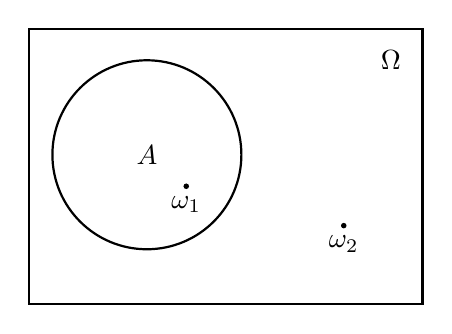
\begin{tikzpicture}[thick]
  \draw (0,0) rectangle (5,3.5);
  \draw (1.5,1.9)node{$A$} circle (1.2);
  \fill (2,1.5) circle(1pt) node[below] {$\omega_1$};
  \fill (4,1) circle(1pt) node[below] {$\omega_2$};
  \node at (4.6,3.1) {$\Omega$};
\end{tikzpicture}
\caption{维恩图\label{fig1.1.1}}
\end{figure}

\begin{example}
  掷一颗骰子的样本空间为:
  $ \Omega = \{1,2,\dotsc,6\}$.

  事件 $A=$“出现 1 点”,
  它由 $\Omega$ 的单个样本点“1”组成.

  事件 $B=$“出现偶数点”,
  它由 $\Omega$ 的三个样本点“2,4,6”组成.

  事件 $C=$“出现的点数小于7”,
  它由的全部样本点“1,2,3,4,5,6”组成,
  即必然事件$\Omega$.

  事件 $D=$“出现的点数大于6”,
  $\Omega$ 中任一样本点都不在 $D$ 中,
  所以 $D$ 是空集,
  即不可能事件 $\emptyset$.
\end{example}

\subsection{随机变量}

用来表示随机现象结果的变量称为\textbf{随机变量}\index{S!随机变量},
常用大写字母 $X$, $Y$, $Z$表示.
很多事件都可用随机变量表示,
表示时应写明随机变量的含义.

\begin{example}
  掷一颗骰子,
  出现的点数是一个随机变量,
  记为 $X$.
  则事件“出现3点”可用“$X = 3$”表示,
  事件“出现的点数不小于3”可用“$X \ge 3$”表示.
  又如“$X < 3$”表示事件“出现点数小于3”.

  掷两颗骰子的样本空间为
  \[
    \Omega =
    \left\{\begin{matrix}
      (1,1) & (1,2) & \dots & (1,6)\\
      (2,1) & (2,2) & \dots & (2,6)\\
      \dots & \dots & \dots & \dots\\
      (6,1) & (6,2) & \dots & (6,6)\\
    \end{matrix}\right\}
  \]
  $\Omega$ 共有 36 个样本点,
  若记 $X$ 与 $Y$ 分别为第一与第二颗骰子出现的点数,
  则 $X$ 与 $Y$ 均可取值:
  1,2,3,4,5,6.
  而事件“点数之和等于5”可表示成
  \[
    “X + Y = 5” = \{(1,4), (2,3), (3,2), (4,1)\}.
  \]

  另外事件“$\max (X,Y) =6$”表示事件“最大点数为6”,
  它含有
  \[
    (1,6),(6,1),(2,6),(6,2),(3,6),(6,3),(4,6),(6,4),(5,6),(6,5),(6,6)
  \]
  共 11 个样本点.
\end{example}

\begin{example}
  检查 10 件产品,
  其中不合格品数 $X$ 是一个随机变量,
  它可以取值 $0,1,\dotsc,10$.
  则事件“不合格品数不多于 1 件”可用“$X \le 1$”来表示. 而“$X>2$”表示事件“不合格品数超过2件”.
\end{example}

\begin{example}
  电视机的寿命 $T$ 是一个随机变量,
  则事件“寿命超过 \SI{40000}{\hour}”可用“$T>40000$”表示,
  而“$T \ge 10000$”表示事件”寿命不超过 \SI{10000}{\hour}”.
\end{example}

在不少场合,
用随机变量表示事件较为简洁明了.
这样一来,
事件有三种表示法:
\begin{enumerate}
  \item 用集合表示.
  \item 用语言表示,
  但语言要明白无误.
  \item 用随机变量表示.
\end{enumerate}
在实际问题中,
哪一种表示法方便就用哪一种.

\subsection{事件间的关系}

下而的讨论总是假设在同一个样本空间 $\Omega$ (即同一个随机现象) 中进行.
事件间的关系与集合间关系一样主要有以下几种:

\subsubsection{包含关系}

如果属于 $A$ 的样本点必属于 $B$,
则称 $A$ 被包含在 $B$ 中 (见图 \ref{fig1.1.2}),
或称 $B$ 包含 $A$,
记为 $A \subset B$,
或 $B \supset A$.
用概率论的语言说:
事件 $A$ 发生必然导致事件 $B$ 发生.

\begin{figure}[!ht]
  \centering
  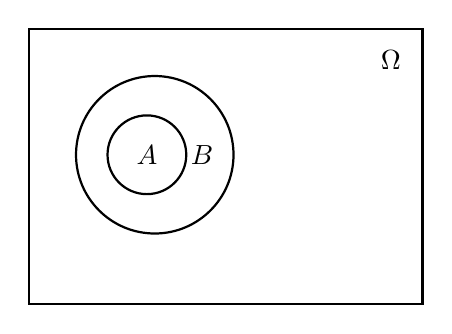
\begin{tikzpicture}[thick]
    \draw (0,0) rectangle (5,3.5);
    \draw (1.5,1.9)node{$A$} circle (0.5);
    \draw (1.6,1.9) circle (1.0);
    \node at (2.2,1.9) {$B$};
    \node at (4.6,3.1) {$\Omega$};
  \end{tikzpicture}
  \caption{$A \subset B$}\label{fig1.1.2}
\end{figure}

譬如掷一颗骰子,
事件 $A=$“出现4点”的发生必然导致事件 $B=$“出现偶数点”的发生,
故 $ A \subset B$.

又如电视机的寿命 $T$ 超过 \SI{10000}{\hour} (记为事件 $A = \{T>10000\}$) 和 $T$ 超过 \SI{20000}{\hour} (记为事件 $B = \{T>20000\}$),
则 $A \supset B$,
见图 \ref{fig1.1.3}.

\begin{figure}[!ht]
  \centering
\begin{tikzpicture}[thick]
  \draw[-Stealth](-1,0) -- (4,0) node[below] {$t$};
  \fill (0,0) node[below] {$0$} circle(1pt);
  \draw (1,0) [bend left=30] to node[above] {$A$} (3.5,1.2);
  \draw (2,0) [bend left=30] to node[below] {$B$} (3.6,0.7);
  \foreach \x in {1,2}
    \draw[fill=white] (\x,0) node[below] {$\x0000$} circle(1pt);
\end{tikzpicture}
  \caption{$\{ T > 10000 \} \supset \{ T > 20000 \}$}\label{fig1.1.3}
\end{figure}

对任一事件 $A$,
必有 $ \emptyset \subset A \subset \Omega $.

\subsubsection{相等关系}

如果事件 $A$ 与事件 $B$ 满足:
属于 $A$ 的样本点必属于 $B$,
而且属于 $B$ 的样本点必属于 $A$,
即 $ A \subset B $ 且 $ B \subset A$,
则称事件 $A$ 与 $B$ 相等,
记为 $A=B$.

从集合论观点看,
两个事件相等就意味着这两事件是同一个集合.
下例说明:
有时不同语言描述的事件也可能是同一件事.

\begin{example}
  \begin{enumerate}
    \item 掷两颗骰子,
    以 $A$ 记事件“两颗骰于的点数之和为奇数”,
    以 $B$ 记事件“两颗骰子的点数为一奇一偶”.
    很容易证明:
    $A$ 发生必然导致 $B$ 发生,
    而且 $B$ 发生也必然导致 $A$ 发生,
    所以 $A=B$.
    \item 口袋中有 $a$ 只黑球,
    $b$ 只白球 ($a$ 与 $b$ 都大于零),
    从中不返回地一只一只摸球.
    以 $A$ 记事件“最后摸出的几个球全是黑球”,
    以 $B$ 记事件“最后摸出的一只球是黑球”.
    对于此题粗看好像是 $A \ne B$,
    但只要设想将球全部摸完为止,
    则明显有:
    $A$ 发生必然会导致 $B$ 发生,
    即 $ A \subset B $;
    反之注意到事件 $A$ 中所述的“几个”最少是1只,
    也可以是2只,
    $\cdots$,
    最多为 $a$ 只,
    则 $B$ 发生时 $A$ 也必然会发生 (对于这点请读者仔细体会),
    即 $B \subset A$,
    由此得 $A=B$.
  \end{enumerate}
\end{example}

\subsubsection{互不相容}

如果 $A$ 与 $B$ 没有相同的样本点 (见图 \ref{fig1.1.4}),
则称 $A$ 与 $B$ 互不相容.
用概率论的语言说:
$A$ 与 $B$ 互不相容就是事件 $A$ 与事件 $B$ 不可能同时发生.

\begin{figure}[!ht]
  \centering
  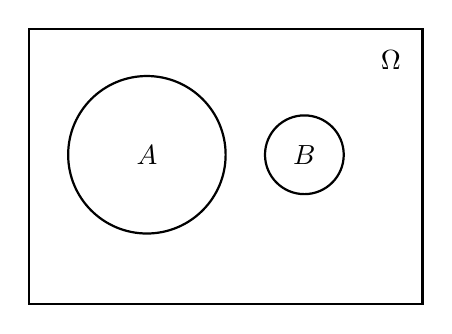
\begin{tikzpicture}[thick]
    \draw (0,0) rectangle (5,3.5);
    \draw (1.5,1.9)node{$A$} circle (1.0);
    \draw (3.5,1.9)node{$B$} circle (0.5);
    \node at (4.6,3.1) {$\Omega$};
  \end{tikzpicture}
  \caption{$A$ 与 $B$ 互不相容}\label{fig1.1.4}
\end{figure}

如在电视机寿命试验中,
“寿命小于1万小时”与“寿命大于5万小时”是两个互不相容的事件,
因为它们不可能同时发生.

\subsection{事件运算}

事件的运算与集合的运算相当,
有并、交、差和余等四种运算.

\subsubsection{事件 $A$ 与 $B$ 的并}
记为 $A \cup B$.
其含义为“由事件 $A$ 与 $B$ 中所有的样本点 (相同的只计入一次) 组成的新事件”(见 图 \ref{fig1.1.5}).
或用概率论的语言说:
“事件 $A$ 与 $B$ 中至少有一个发生”.

\begin{figure}[!ht]
  \centering
  \begin{tikzpicture}[thick]
    \draw (0,0) rectangle (5,3.5);
    \fill[pattern=north west lines]
      (1.5,1.9) circle (1) (2.8,1.9) circle(0.8);
    \draw (1.5,1.9)node[inner sep=0pt,fill=white]{$A$} circle (1);
    \draw (2.8,1.9)node[inner sep=0pt,fill=white]{$B$} circle(0.8);
    \node at (4.6,3.1) {$\Omega$};
  \end{tikzpicture}
  \caption{$A$ 与 $B$ 的并}\label{fig1.1.5}
\end{figure}

如在掷一颗骰子的试验中,
记事件 $A=$“出现奇数点”$=\{1,3,5\}$,
记事件 $B=$“出现的点数不超过3”$=\{1,2,3\}$,
则 $A$ 与 $B$ 的并为 $A \cup B = \{1,2,3,5\}$.

\subsubsection{事件 $A$ 与 $B$ 的交}

记为 $A \cap B$,
或简记为 $AB$.
其含义为“由事件 $A$ 与 $B$ 中公共的样本点组成的新事件”(见图 \ref{fig1.1.6})).
或用概率论的语言说:
“事件 $A$ 与 $B$ 同时发生”.

\begin{figure}[!ht]
  \centering
  \begin{tikzpicture}[thick]
    \draw (0,0) rectangle (5,3.5);
    \begin{scope}
    \clip(1.5,1.9) circle (1);
    \fill[pattern=north west lines] (2.8,1.9) circle(0.8);
    \end{scope}
    \draw (2.8,1.9) circle(0.8);
    \draw (1.5,1.9)node{$A$} circle (1);
    \draw (2.8,1.9)node{$B$} circle(0.8);
    \node at (4.6,3.1) {$\Omega$};
  \end{tikzpicture}
  \caption{$A$ 与 $B$ 的交}\label{fig1.1.6}
\end{figure}

如在掷一颗骰子的试验中,
记事件 $A=$“出现奇数点”$=\{1,3,5\}$,
记事件 $B=$“出现的点数不超过3”$=\{1,2,3\}$,
则 $A$ 与 $B$ 的交为 $AB = \{1,3\}$.

若事件 $A$ 与 $B$ 为互不相容,
则其交必为不可能事件,
即 $AB = \emptyset$,
反之亦然.
这表明:
$AB = \emptyset$ 就意味着 $A$ 与 $B$ 是互不相容事件.

事件的并与交运算可推广到有限个或可列个事件,
譬如有事件 $A_1$, $A_2$, $\dotsc$,
则 $\bigcup_{i=1}^n A_i$ 称为有限并;
$\bigcup_{i=1}^{+\infty} A_i$ 称为可列并;
$\bigcap_{i=1}^n A_i$ 称为有限交;
$\bigcup_{i=1}^{+\infty} A_i$ 称为可列交.

\subsubsection{事件 $A$ 对 $B$ 的差}

记为 $A-B$,
其含义为“由事件 $A$ 中而不在 $B$ 中的样本点组成的新事件”(见图 \ref{fig1.1.7}).
或用概率论的语言说:
“事件 $A$ 发生而 $B$ 不发生”.

\begin{figure}[!ht]
  \centering
  \begin{subfigure}{0.4\linewidth}
    \centering
    \begin{tikzpicture}[thick]
    \draw (0,0) rectangle (5,3.5);
    \fill[pattern=north west lines](1.5,1.9) circle (1);
    \filldraw[fill=white,draw=black] (2.8,1.9)node{$B$} circle(0.8);
    \draw (1.5,1.9)node[inner sep=0pt,fill=white]{$A$} circle (1);
    \node at (4.6,3.1) {$\Omega$};
  \end{tikzpicture}
    \caption{$A-B$}
  \end{subfigure}
  \begin{subfigure}{0.4\linewidth}
    \centering
    \begin{tikzpicture}[thick]
    \draw (0,0) rectangle (5,3.5);
    \filldraw[pattern=north west lines,draw=black](2,1.9)node
    [fill=white,inner sep=0pt]{$A$} circle (1);
    \filldraw[fill=white,draw=black] (1.5,1.9)node{$B$} circle(0.3);
    \node at (4.6,3.1) {$\Omega$};
  \end{tikzpicture}
    \caption{$A-B(A \supset B)$}
  \end{subfigure}
  \caption{}\label{fig1.1.7}
\end{figure}

如在掷一颗骰子的试验中,
记事件 $A=$“出现奇数点”$=\{1,3,5\}$,
记事件 $B=$“出现的点数不超过3”$=\{1,2,3\}$,
则 $A$ 对 $B$ 的差为 $A-B=\{15\}$.

若设 $X$ 为随机变量,
则有
\[
  \{ X = a \}
  = \{ X \le a \} - \{ X < a \},
  \quad
  \{ a < X \le b \}
  = \{ X \le b \} - \{ X \le a \}.
\]

\subsubsection{对立事件}

事件 $A$ 的对立事件,
记为 $\overline{A}$,
即“由在 $\Omega$ 中而不在 $A$ 中的样本点组成的新事件”(见图 \ref{fig1.1.8}),
或用概率论的语言说:
“$A$ 不发生”,
即 $\overline{A} = \Omega - A$.
注意,
对立事件是相互的,
即 $A$ 的对立事件是 $\overline{A}$,
而 $\overline{A}$ 的对立事件是 $A$,
即 $\overline{\overline{A}}=A$.
必然事件 $\Omega$ 与不可能事件 $\emptyset$ 互为对立事件,
即 $\overline{\Omega} = \emptyset$,
$\overline{\emptyset} = \Omega$.

\begin{figure}[!ht]
  \centering
  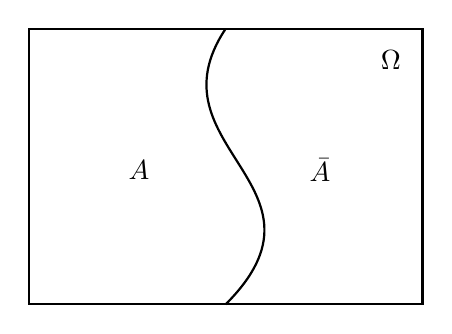
\begin{tikzpicture}[thick]
    \draw (0,0) rectangle (5,3.5);
    \node at (4.6,3.1) {$\Omega$};
    \draw (2.5,0).. controls (4,1.5) and (1.5,2)..(2.5,3.5);
    \draw (1.4,1.7)node{$A$} (3.7,1.7)node{$\bar A$};
  \end{tikzpicture}
  \caption{$A$ 的对立事件 $\overline{A}$}\label{fig1.1.8}
\end{figure}

如在掷一颗骰子的试验中,
事件 $A=$“出现奇数点”$= \{1,3,5\}$ 的对立事件是 $\overline{A} = \{2,4,6\}$,
事件 $B=$“出现的点数不超过3”$= \{1,2,3\}$ 的对立事件是 $\bar B =
\{4,5,6\}$.

$A$ 与 $B$ 互为对立事件的充要条件是:
$A \cap B = \emptyset$,
且 $A \cup B = \Omega$.

此性质也可作为对立事件的另一种定义,
即如果事件 $A$ 与 $B$ 满足:
$A \cap B = \emptyset$,
且 $A \cup B = \Omega$,
则称 $A$ 与 $B$ 互为对立事件,
记为 $\overline{A} = B$,
$\overline{B} = A$.

\begin{example}
  从数字$ 1, 2,\cdots, 9$ 中可重复地任取 $n$ 次 ($n \ge 2$),
  以 $A$ 表示事件“所取的 $n$ 个数字的乘积能被10整除”.
  因为乘积能被 10 整除必须既取到数字 5,
  又要取到偶数.
  所以 $A$ 的对立事件 $\overline{A}$ 为“所取的 $n$ 个数字中或者没有 5,
  或者没有偶数”.
  如果记 $B=$“所取的 $n$ 个数字中没有5”,
  $C=$“所取的 $n$ 个数字中没有偶数”,
  则 $\overline{A} = B \cup C$.
\end{example}

\begin{example}
  设 $A$、$B$、$C$ 是某个随机现象的三个事件,
  则
  \begin{enumerate}
    \item 事件“$A$ 与 $B$ 发生,
    $C$ 不发生”可表示为: $AB\overline{C}$.
    \item 事件“$A$、$B$、$C$ 中至少有一个发生”可表示为: $A \cup B \cup C$.
    \item 事件“$A$、$B$、$C$ 中至少有两个发生”可表示为: $AB \cup AC \cup BC$.
    \item 事件“$A$、$B$、$C$ 中恰好有两个发生”可表示为: $AB\overline{C} \cup A\overline{B}C \cup \overline{A}BC$.
    \item 事件“$A$、$B$、$C$ 同时发生”可表示为: $ABC$.
    \item 事件“$A$、$B$、$C$ 都不发生”可表示为: $\overline{A}\overline{B}\overline{C}$.
    \item 事件“$A$、$B$、$C$ 不全发生”可表示为: $\overline{A} \cup \overline{B} \cup \overline{C}$.
  \end{enumerate}
\end{example}

\subsubsection{事件的运算性质}
\begin{enumerate}
  \item 交换律
  \begin{equation}\label{eq1.1.1}
    A \cup B = B \cup A, \quad AB = BA
  \end{equation}
  \item 结合律
  \begin{gather}
    (A \cup B) \cup C = A \cup (B \cup C),\label{eq1.1.2}\\
    (AB)C = A(BC).\label{eq:1.1.3}
  \end{gather}
  \item 分配律
  \begin{gather}
    (A \cup B) \cup C = A \cup (B \cup C),\label{eq1.1.4}\\
    (A \cap B) \cup C = (A \cup C) \cap (B \cup C).\label{eq1.1.5}
  \end{gather}
  \item 对偶律 (德莫根公式)
  \begin{gather}
    \text{事件并的对立等于对立的交:} \quad \overline{A \cup B} = \overline{A} \cap \overline{B},\label{eq1.1.6}\\
    \text{事件交的对立等于对立的并:} \quad \overline{A \cap B} = \overline{A} \cup \overline{B}.\label{eq1.1.7}
  \end{gather}
\end{enumerate}

事件运算的对偶律是很有用的公式.
这些性质是不难证明的,
在此我们用集合论的语言证明其中的 \eqref{eq1.1.6} 式.

\subsubsection*{\eqref{eq1.1.6} 式的证明}

设 $\omega \in \overline{A \cup B}$,
即 $\omega \notin A \cup B$,
这表明 $\omega$ 既不属于 $A$,
也不属于 $B$,
这意味着 $\omega \notin A$ 和 $\omega \notin B$ 同时成立,
所以 $\omega \in \overline{A}$ 与 $\omega \in \overline{B}$ 同时成立,
于是有 $\omega \in \overline{A} \cap \overline{B}$,
这说明
\[
  \overline{A \cup B} \subset \overline{A} \cap \overline{B}.
\]

反之,
设 $\omega \in \overline{A} \cap \overline{B}$,
即同时有 $\omega \in \overline{A}$ 和$\omega \in \overline{B}$,
从而同时有 $\omega \notin A$ 和 $\omega \notin B$,
这意味着 $\omega$ 不属于 $A$ 与 $B$ 中的任一个,
即 $\omega \notin A \cup B$,
也就是有 $\omega \in \overline{A \cup B}$,
这说明
\[
  \overline{A \cup B} \supset \overline{A} \cap \overline{B}.
\]

综合上述两方面,
可得
\[
  \overline{A \cup B} = \overline{A} \cap \overline{B}.
\]
\eqref{eq1.1.6} 式得证.

德莫根公式可推广到多个事件及可列个事件场合:
\begin{gather}
  \overline{\bigcup _{i=1} ^n A _i} = \bigcap _{i=1} ^n \overline{A} _i;
  \quad \overline{\bigcup _{i=1} ^{+\infty} A _i} = \bigcap _{i=1} ^{+\infty} \overline{A} _i; \label{eq1.1.8}\\
  \overline{\bigcap _{i=1} ^n A _i} = \bigcup _{i=1} ^n \overline{A} _i;
  \quad \overline{\bigcap _{i=1} ^{+\infty} A _i} = \bigcup _{i=1} ^{+\infty} \overline{A} _i. \label{eq1.1.9}
\end{gather}

\subsection{事件域}

在此我们要给出的“事件域”概念,
目的是为下一节定义事件的概率作准备.

所谓的“事件域”从直观上讲就是一个样本空间中某些子集组成的集合类,
以后记事件域为 $\mathscr{F}$.

当样本空间是实数轴上的一个区间时,
可以人为地构造出无法测量其长度的子集,
这样的子集常被称为不可测集.
如果将这些不可测集也看成是事件,
那么这些事件将无概率可言,
这是我们不希望出现的现象,
为了避兔这种现象出现,
我们没有必要将连续样本空间的所有子集都看成是事件,
只需将我们感兴趣的子集 (又称\textbf{可测集})\index{K!可测集} 看成是事件即可.

现在的问题是:
我们应该对哪些子集感兴趣,
或换句话说,
$\mathscr{F}$ 中应该有哪些元素?
首先 $\mathscr{F}$ 应该包括 $\Omega$ 和 $\emptyset$;
其次应该保证事件经过前面所定义的各种运算 (并、交、差、对立) 后仍然是事件,
即 $\mathscr{F}$ 要对集合的运算有封闭性.
经过研究人们发现
\begin{itemize}
  \item 交的运算可通过并与对立来实现 (德莫根公式).
  \item 差的运算可通过对立与交来实现 ($A - B = A\overline{B}$).
\end{itemize}

这样一来,
可给出事件域的定义如下.


\begin{definition}{}{1.1.1}
  设 $ \Omega $ 为一样本空间,
  $\mathscr{F}$ 为 $\Omega$ 的某些子集所组成的集合类,
  如果 $\mathscr{F}$ 满足:
  \begin{enumerate}
      \item $\Omega \in \mathscr{F}$;
      \item 若 $A \in \mathscr{F}$, 则对立事件 $\overline{A} \in \mathscr{F}$;
      \item 若 $A _n \in \mathscr{F}$, $1,2,\dotsc$, 则可列并 $\bigcup _{n=1} ^{+\infty} A _n \in \mathscr{F}$.
  \end{enumerate}
  则称 $\mathscr{F}$ 为一个\textbf{事件域}, \index{S!随机事件!事件域}
  又称为 \textbf{$\sigma$ 代数}. \index{S!随机事件!$\sigma$代数}
\end{definition}

在概率论中,
又称 $(\Omega, \mathscr{F})$ 为\textbf{可测空间},\index{S!随机事件!可测空间}
这里“可测”是指 $\mathscr{F}$ 中都是有概率可言的事件.

\begin{example}
  常见的事件域
  \begin{enumerate}
    \item 若样本空间只含两个样本点: $\Omega = \{\omega_1, \omega_2\}$, 记 $A = \{\omega_1\}$, $\overline{A} = \{\omega_2\}$, 则其事件域为 $\mathscr{F} = \{\emptyset, A, \overline{A}, \Omega\}$.
    \item 若样本空间含有 $n$ 个样本点: $\Omega = \{\omega_1, \omega_2, \dotsc, \omega_n\}$, 则其事件域 $\mathscr{F}$ 是由空集 $\emptyset$、$n$ 个单元素集、$\binom{n}{2}$ 个双元素集、$\binom{n}{3}$ 个三元素集……和 $\Omega$ 组成的集合类, 这时 $\mathscr{F}$ 中共有 $\binom{n}{0} + \binom{n}{1} + \binom{n}{2} + \dotsb + \binom{n}{n} = 2^n$ 个事件.
    \item 若样本空间含有可列个样本点: $\Omega = \{\omega_1, \omega_2, \dotsc, \omega_n, \dotsc\}$, 则其事件域 $\mathscr{F}$ 是由空集 $\emptyset$、可列个单元素集、可列个双元素集……可列个 $n$ 个元素集……和 $\Omega$ 组成的集合类, 这时 $\mathscr{F}$ 是由可列个的可列个 (仍为可列个) 元素 (事件) 组成.
    \item 若样本空间含有全体实数: $\Omega = (-\infty, +\infty) = \mathbb{R}$. 这时事件域 $\mathscr{F}$ 中的元素无法一一列出, 而是由一个基本集合类逐步扩展形成, 具体操作如下:
    \begin{itemize}
      \item 取基本集合类 $\mathscr{F} =$“全体半直线组成的类”, 即
      \[ \mathscr{F} = \{(-\infty, x); -\infty < x < +\infty\}.\]
      \item 利用事件域的要求, 首先把有限的左闭右开区间扩展进来:
      \[ [a, b) = (-\infty, b) - (\infty, a), \quad \text{其中 } a, b \text{ 为任意实数}. \]
      \item 再把闭区间、单点集、左开右闭区间、开区间扩展进来:
      \[ [a,b] = \bigcap _{n=1} ^{+\infty} [a, b + 1/n), \]
      \[ \{b\} = [a, b] - [a, b), \]
      \[ (a, b] = [a, b] - \{a\}, \]
      \[ (a, b) = [a, b) - \{a\}. \]
      \item 最后用 (有限个或可列个) 并运算和交运算把实数集中一切有限集、可列集、开集、闭集都扩展进来.
    \end{itemize}

    经过上述几步扩展所得之集的全体就是人们希望得到的事件域 $\mathscr{F}$,
    因为它满足事件城的定义.
    这样的事件域 $\mathscr{F}$ 又称为\textbf{波雷尔 (Borel) 事件城},\index{S!随机事件!波雷尔 事件域}
    域中的每个元素 (集合)又称为波雷尔集,
    或称为可测集,
    这种可测集都是有概率可言的事件.
  \end{enumerate}
\end{example}

\begin{xiti}
  \item 写出下列随机试验的样本空间:
  \begin{enumerate}
    \item 抛三枚硬币;
    \item 抛三颗骰子;
    \item 连续抛一枚硬币, 直至出现正为之;
    \item 在某十字路口, 一小时内通过的机动车辆数;
    \item 某城市一天内的用电量.
  \end{enumerate}

  \item 在抛三枚硬币的试验中写出下列事件的集合表示:
  \begin{itemize}
    \item $A =$“至少出现一个正面”;
    \item $B =$“最多出现一个正面”;
    \item $C =$“恰好出现一个正面”;
    \item $D =$“出现三面相同”.
  \end{itemize}

  \item 设 $A$、$B$、$C$ 为三事件, 试表示下列事件:
  \begin{enumerate}
    \item $A$、$B$、$C$ 都发生或都不发生;
    \item $A$、$B$、$C$ 中不多于一个发生;
    \item $A$、$B$、$C$ 中不多于两个发生;
    \item $A$、$B$、$C$ 中至少有两个发生.
  \end{enumerate}

  \item 请指明以下事件 $A$ 和 $B$ 间的关系:
  \begin{enumerate}
    \item 检查两件产品, 记事件 $A =$“至少有一件不合格产品”, $B =$“两次检查结果不同”.
    \item 设 $T$ 表示轴承寿命, 记事件 $A = \{T > \text{\SI{5000}{\hour}}\}$, $B = \{T > \text{\SI{8000}{\hour}}\}$.
  \end{enumerate}

  \item 设 $X$ 为随机变量, 其样本空间为 $\Omega = \{0 \le T \le 2\}$, 记事件 $A =\{0.5 < X \le 1\}$, $B = \{0.25 \le X < 1.5\}$. 写出下列事件:
  \begin{enumerate}
    \item $\overline{A}B$,
    \item $\overline{A} \cup B$,
    \item $\overline{AB}$,
    \item $\overline{A \cup B}$.
  \end{enumerate}

  \item 对飞机进行两次射击, 每次射一弹, 设 $A = \{$恰有一弹击中飞机$\}$, $B = \{$至少有弹击中飞机$\}$, $C = \{$两弹都击中飞机$\}$, $D = \{$两弹都没击中飞机$\}$. 又设随机变量 $X$ 为击中飞机的次数, 试用 $X$ 表示事件 $A$, $B$, $C$, $D$. 进一步问 $A$, $B$, $C$, $D$ 中哪些是互不相容的事件? 哪些是对立的事件?

  \item 试问下列命题是否成立?
  \begin{enumerate}
    \item $ A - (B - C) = (A - B) \cup C.$
    \item 若 $AB = \emptyset$ 且 $ C \subset A$, 则 $BC = \emptyset$.
    \item $(A \cup B) - B = A$.
    \item $(A - B) \cup B = A$.
  \end{enumerate}

  \item 试用维恩图说明, 当事件 $A$ 与 $B$ 互不相容时, 能否得出结论 $\overline{A}$ 与 $\overline{B}$ 相容.

  \item 请叙述下列事件的对立事件:
  \begin{enumerate}
    \item $A = $“掷两枚硬币, 皆为正面”;
    \item $B = $“射击三次, 皆命中目标”;
    \item $C = $“加工四个零件, 至少有一个合格品”.
  \end{enumerate}

  \item 如果 $A$ 与 $B$ 互为对立事件, 证明: $\overline{A}$ 与 $\overline{B}$ 也互为对立事件.

  \item 设 $\mathscr{F}$ 为一事件域, 若 $A_n \in \mathscr{F}$, $n = 1,2, \dotsc$, 试证:
  \begin{enumerate}
    \item $\emptyset \in \mathscr{F}$;
    \item 有限并 $\bigcup _{i=1}^n A_i \in \mathscr{F}$, $n \ge 1$;
    \item 有限交 $\bigcap _{i=1}^n A_i \in \mathscr{F}$, $n \ge 1$;
    \item 可列交 $\bigcap _{i=1}^{+\infty} A_i \in \mathscr{F}$;
    \item 差运算 $A_1 - A_2 \in \mathscr{F}$.
  \end{enumerate}
\end{xiti}

\section{概率的定义及其确定方法}

在这一节中,
我们要给出概率的定义及其确定方法,
这是概率论中最基本的个问题.
简单而直观的说法就是:
概率是随机事件发生的可能性大小,
对此我们先看下面一些经验事实:
\begin{enumerate}
  \item 随机事件的发生是带有偶然性.
  但随机事件发生的可能性是有大小之分的,
  例如口袋中有10只相同大小的球,
  其中9只黑球,
  1只红球,
  从口袋中任取1球,
  人们的共识是:
  取出黑球的可能性比取出红球的可能性大;
  \item 随机事件发生的可能性是可以设法度量的,
  就好比一根木棒有长度,
  一块土地有面积一样.
  例如抛一枚硬币,
  出现正面与出现反面的可能性是相同的,
  各为 $1/2$.
  足球裁判就用抛硬币的方法让双方队长选择场地,
  以示机会均等;
  \item 在日常生活中,
  人们对一些随机事件发生的可能性大小往往是用百分比 (0到1之间的一个数) 进行度量的.
  例如购买彩券后可能中奖,
  可能不中奖,
  但中奖的可能性大小可以用中奖率来度量;
  抽取一个产品可能为合格品,
  也可能为不合格品,
  但产品质量的好坏可以用不合格品率来度量;
  新生要儿可能为男孩,
  也可能为女孩,
  但生男孩的可能性可以用男婴出生率来度量.
\end{enumerate}

在概率论发展的历史上,
曾有过概率的古典定义、概率的几何定义、概率的频率定义和概率的主观定义.
这些定义各适合一类随机现象,
那么如何给出适合一切随机现象的概率的最一般的定义呢?
1900年数学家希尔伯特 (1862-1943) 提出要建立概率的公理化定义以解决这个问题,
即以最少的几条本质特性出发去刻画概率的概念.
1933年前苏联数学家柯尔莫哥洛夫 (1903-1987) 首次提出了概率的公理化定义,
这个定义既概括了历史上几种概率定义中的共同特性,
又避免了各自的局限性和含混之处,
不管什么随机现象,
只有满足定义中的三条公理,
才能说它是概率.
这一公理化体系迅速获得举世公认,
是概率论发展史上的一个里程碑.
有了这个公理化定义后,
概率论得到了很快的发展.

\subsection{概率的公理化定义}

\begin{definition}{}{1.2.1}
  设 $\Omega$ 为一个样本空间,
  $\mathscr{F}$ 为 $\Omega$ 的某些子集组成的一个事件域.
  如果对任一事件 $A \in \mathscr{F}$,
  定义在 $\mathscr{F}$ 上的一个实值函数 $P(A)$ 满足:
  \begin{enumerate}
    \item 非负性公理:
    若 $A \in \mathscr{F}$,
    则 $P(A) \ge 0$;
    \item 正则性公理:
    $P (\Omega) = 1$;
    \item 可列可加性公理:
    若 $A_1$, $A_2$, \dots, $A_n$, \dots, 互不相容,
    有
    \begin{equation}
      P \biggl( \bigcup _{i=1} ^{+\infty} A_i \biggr) = \sum _{i=1} ^{+\infty} P ( A _i ),\label{eq1.2.1}
    \end{equation}
  \end{enumerate}
  则称 $P (A)$ 为事件 $A$ 的概率,
  称三元素 $(\Omega, \mathscr{F}, \mathscr{P})$ 为\textbf{概率空间}.
\end{definition}

概率的公理化定义刻画了概率的本质,
概率是集合 (事件) 的函数,
若在事件域 $\mathscr{F}$ 上给出一个函数,
当这个函数能满足上述三条公理,
就被称为概率;
当这个函数不能满足上述三条公理中任一条,
就被认为不是概率.

公理化定义没有告诉人们如何去确定概率.
历史上在公理化定义出现之前概率的频率定义、古典定义、几何定义和主观定义都在一定的场合下,
有着各自确定概率的方法,
所以在有了概率的公理化定义之后,
把它们看作确定概率的方法是恰当的.
下面先介绍在确定概率的古典方法中大量使用的排列与组合公式,
然后分别讲述确定概率的方法.

\subsection{排列与组合公式}

排列与组合都是计算“从 $n$ 个元素中任取 $r$ 个元素”的取法总数公式,
其主要区别在于:
如果不讲究取出元素间的次序,
则用组合公式,
否则用排列公式;
而所谓讲究元素间的次序,
可以从实际问题中得以辨别,
例如两个人相互握手是不讲次序的,
而两个人排队是讲次序的,
因为“甲右乙左”与“乙右甲左”是两件事.

排列与组合公式的推导都基于如下两条计数原理:
\begin{enumerate}
  \item 乘法原理:
  如果某件事经 $k$ 个步骤才能完成,
  做第一步有 $m_1$ 种方法,
  做第二步有 $m_2$ 种方法,
  \dots,
  做第 $k$ 步有 $m_k$ 种方法.
  那么完成这件事共有 $m_1 \times m_2 \times \dotsb \m_k$ 种方法.

  譬如,
  甲城到乙城有3条旅游线路,
  由乙城到丙城有2条旅游线路,
  那么从甲城经乙城去丙城共有 $3 \times 2 = 6$ 条旅游线路.

  \item 加法原理:
  如果某件事可由 $k$ 类不同途径之一去完成,
  在第一类途径中有 $m_1$ 种完成方法,
  在第二类途径中有 $m_2$ 种完成方法,
  \dots,
  在第 $k$ 类途径中有 $m_k$ 种完成方法,
  那么完成这件事共有 $m_1 + m_2 + \dotsb + m_k$ 种方法.

  譬如,
  由甲城到乙城去旅游有三类交通工具:
  汽车、火车和飞机.
  而汽车有5个班次,
  火车有3个班次,
  飞机有2个班次,
  那么从甲城到乙城共有 $5 + 3 + 2 = 10$ 个班次供旅游者选择.
\end{enumerate}

排列与组合的定义及其计算公式如下.
\begin{enumerate}
  \item 排列:
  从 $n$ 个不同元素中任取 $r (r \le n)$ 个元素排成一列 (考虑元素先后出现次序),
  称此为一个排列,
  此种排列的总数记为 $P_n^r$,
  按乘法原理,
  取出的第一个元素有 $n$ 种取法,
  取出的第二个元素有 $n - 1$ 种取法\dots
  取出的第 $r$ 个元素有 $n - r + 1$ 种取法,
  所以有
  \begin{equation}
    P_n^r = n \times (n - 1) \times \dotsb \times (n - r + 1) = \frac{n!}{(n - r!)}.\label{eq1.2.2}
  \end{equation}
  若 $r = n$,
  则称为全排列,
  记为 $_n$.
  显然,
  全排列 $P_n = n!$.

  \item 重复排列:
  从 $n$ 个不同元素中每次取出一个,
  放回后再取下一个,
  如此连续取 $r$ 次所得的排列称为重复排列,
  此种重复排列数共有 $n^r$ 个.
  注意这里的 $r$ 允许大于 $n$.

  \item 组合:
  从 $n$ 个不同元素中任取 $r (r \le n)$ 个元素并成一组 (不考虑元素间的先后次序),
  称此为一个组合,
  此种组合的总数记为 $\binom{n}{r}$ 或 $C_n^r$.
  按乘法原理此种组合的总数为
  \begin{equation}
    \binom{n}{r} = \frac{P_n^r}{r!} = \frac{n (n - 1) \dotsb (n - r + 1)}{r!} = \frac{n!}{r! (n - r)!}.\label{eq1.2.3}
  \end{equation}
  在此规定 $0! = 1$ 与 $\binom{n}{0} = 1$.

  \item 重复组合:
  从 $n$ 个不同元素中每次取出一个,
  放回后再取下一个,
  如此连续取 $r$ 次所得的组合称为重复组合,
  此种重复组合总数为 $\binom{n + r - 1}{r}$.
  注意这里的 $r$ 也允许大于 $n$.
\end{enumerate}

上述四种排列组合及其总数计算公式,
在确定概率的古典方法中经常使用,
但在使用中要注意识别有序与无序、重复与不重复。

\subsection{确定概率的频率方法}

确定概率的频率方法是一种最常用的方法,
其基本思想是:
\begin{enumerate}
  \item 与考察事件 $A$ 有关的随机现象可大量重复进行.
  \item 在 $n$ 次重复试验中,
  记 $n (A)$ 为事件 $A$ 出现的次数,
  又称 $n (A)$为事件 $A$ 的\textbf{频数},
  称
  \begin{equation}
    f_n (A) = \frac{n (A)}{n}\label{eq1.2.4}
  \end{equation}
  为事件 $A$ 出现的\textbf{频率}.

  \item 人们的长期实践表明:
  随着试验重复次数 $n$ 的增加,
  频率 $f_n (A)$ 会稳定在某一常数 $a$ 附近.
  我们称这个常数为\textbf{频率的稳定值}.
  这个频率的稳定值就是我们所求的概率.

  \item 频率方法的缺点是:
  在现实世界里,
  人们无法把一个试验无限次地重复下去,
  因此要精确获得频率的稳定值是困难的.
  但频率方法提供了概率的一个可供想像的具体值,
  并且在试验重复次数 $n$ 较大时,
  可用频率给出概率的一个近似值,
  这一点是频率方法最有价值的地方.
  在统计学中就是如此做的,
  且称频率为概率的估计值.
\end{enumerate}

容易验证:
用频率方法确定的概率满足公理化定义,
它的非负性与正则性是显然的,
而可加性只需注意到:
当 $A$ 与 $B$ 互不相容时,
计算 $A \cup B$ 的频数可以分别计算的 $A$ 的频数和 $B$ 的频数,
然后再相加,
这意味着 $n (A \cup B) = n (A) + n (B)$.
从而有
\begin{align*}
  f _n (A \cup B) &= \frac{n (A \cup B)}{n} = \frac{n (A) + n (B)}{n}\\
  &= \frac{n (A)}{n} + \frac{n (B)}{n} = f _n (A) + f _n (B).
\end{align*}

\begin{example}
  说明频率稳定性的例子.
  \begin{enumerate}
    \item 抛硬币试验

    历史上有不少人做过抛硬币试验,
    其结果见表~\ref{tab1.2.1}.
    从表中的数据可以看出:
    出现正面的频率逐渐稳定在0.5,
    用频率的方法可以说:
    出现正面的概率为0.5.

    \begin{table}[h]
      \centering
      \caption{历史上抛硬币试验的若干结果}\label{tab1.2.1}
      \begin{tabularx}{0.9\linewidth}{*{4}{X}}
        \toprule
        实验者 & 抛硬币次数 & 出现正面次数 & 频率\\
        \midrule
        德莫根 (De morgan) & 2048 & 1061 & 0.5181\\
        蒲丰 (Buffon) & 4040 & 2048 & 0.5069\\
        费勒 (Feller) & 10000 & 4979 & 0.4979\\
        皮尔逊 (Pearson) & 12000 & 6019 & 0.5016\\
        皮尔逊 & 24000 & 12012 & 0.5005\\
        \bottomrule
      \end{tabularx}
    \end{table}

    \item 英语字母的频率

    人们在生活实践中已经认识到:
    英语中某些字母出现的频率要高于另外一些字母.
    但26个英文字母各自出现的频率到底是多少?
    有人对各类典型的英语书刊中字母出现的频率进行统计,
    发现各个字母的使用频率相当稳定 (见表~\ref{tab1.2.2}).
    这项研究对计算机键盘的设计 (在方便的地方安排使用频率最高的宇母键)、信息的编码 (用较短的码编排使用频率最高的字母键) 等等方面都是十分有用的.

    \begin{table}[h]
      \centering
      \caption{英文字母的使用率}\label{tab1.2.2}
      \begin{tabularx}{0.9\linewidth}{*{6}{Z}}
        \toprule
        字母 & 使用频率 & 字母 & 使用频率 & 字母 & 使用频率\\
        \midrule
        E & 0.1268 & L & 0.0394 & P & 0.0186\\
        T & 0.0978 & D & 0.0389 & B & 0.0156\\
        A & 0.0788 & U & 0.0280 & V & 0.0102\\
        O & 0.0776 & C & 0.0268 & K & 0.0060\\
        I & 0.0707 & F & 0.0256 & X & 0.0016\\
        N & 0.0706 & M & 0.0244 & J & 0.0010\\
        S & 0.0634 & W & 0.0214 & Q & 0.0009\\
        R & 0.0594 & Y & 0.0202 & Z & 0.0006\\
        H & 0.0573 & G & 0.0187 &   &       \\
        \bottomrule
      \end{tabularx}
    \end{table}

    \item 女婴出生频率

    研究女婴出生频率,
    对人口统计是很重要的.
    历史上较早研究这个问题的有拉普拉斯 (1794-1827),
    他对伦敦、彼得堡、柏林和全法国的大量人口资料进行研究,
    发现女要出生频率总是在 $21/43$ 左右波动.

    统计学家克拉梅 (1893-1985) 用瑞典 1935 年的官方统计资料 (见表~\ref{tab1.2.3}),
    发现女要出生频率总是在 0.482 左右波动.

    \begin{table}[h]
      \centering
      \caption{瑞典 1935 年各月出生女的频率}\label{tab1.2.3}
      \begin{tabularx}{0.9\linewidth}{*{8}{Z}}
        \toprule
        月份 & 1 & 2 & 3 & 4 & 5 & 6 & \\
        \midrule
        婴儿数 & 7280 & 6957 & 7883 & 7884 & 7892 & 7609 &\\
        女婴数 & 3537 & 3407 & 3866 & 3711 & 3775 & 3665 &\\
        频率 & 0.486 & 0.489 & 0.490 & 0.471 & 0.478 & 0.482 &\\
        \midrule
        \midrule
        月份 & 7 & 8 & 9 & 10 & 11 & 12 & 全年\\
        \midrule
        婴儿数 & 7585 & 7393 & 7203 & 6903 & 6552 & 7132 & 88273\\
        女婴数 & 3621 & 3596 & 3491 & 3391 & 3160 & 3371 & 42591\\
        频率 & 0.462 & 0.484 & 0.485 & 0.491 & 0.482 & 0.473 & 0.4825\\
        \bottomrule
      \end{tabularx}
    \end{table}
  \end{enumerate}
\end{example}

\subsection{确定概率的古典方法}

确定概率的古典方法是概率论历史上最先开始研究的情形.
它简单、直观,
不需要做大量重复试验,
而是在经验事实的基础上,
对被考察事件的可能性进行逻辑分析后得出该事件的概率.

古典方法的基本思想如下:
\begin{enumerate}
  \item 所涉及的随机现象只有有限个样本点,
  譬如为 $n$ 个.
  \item 每个样本点发生的可能性相等 (称为等可能性).
  例如,
  抛一枚均匀硬币,
  “出现正面”与“出现反面”的可能性相等;
  抛一枚均匀骰子,
  出现各点 (1--6) 的可能性相等;
  从一副扑克牌中任取一张,
  每张牌被取到的可能性相等.

  \item 若事件 $A$ 含有 $k$ 个样本点,
  则事件 $A$ 的概率为
  \begin{equation}
    P (A) = \frac{\text{事件 } A \text{ 所含样本点的个数}}{\Omega \text{ 中所有样本点的个数}}
    = \frac{k}{n}.\label{eq1.2.5}
  \end{equation}
\end{enumerate}

容易验证,
由上式确定的概率满足公理化定义,
它的非负性与正则性是显然的;
而满足可加性的理由与频率方法类似:
当 $A$ 与 $B$ 互不相容时,
计算 $A \cup B$ 的样本点个数可以分别计算 $A$ 的样本点个数和 $B$ 的样本点个数,
然后再相加,
从而有可加性 $P (A \cup B) = P (A) + P (B) $.

在古典方法中,
求事件 $A$ 的概率主要是计算 $A$ 中含有的样本点的个数和 $\Omega$ 中含有的样本点的个数.
所以在计算中经常用到排列组合工具.

\begin{example}
  掷两枚硬币,
  求出现一个正面一个反面的概率.
\end{example}

\begin{solution}
  此例的样本空间为 $\Omega = \{ (\text{正}, \text{正})$, $(\text{正}, \text{反})$, $(\text{反}, \text{正})$, $(\text{反}, \text{反}) \}$.
  所以 $\Omega$ 中含有样本点的个数为4,
  事件“出现一个正面一个反面”含有的样本点的个数为2个,
  因此所求概率为 1/2.
\end{solution}

注意,
如果将此样本空间记成 $\Omega = \{ (\text{二正})$, $(\text{二反})$, $(\text{一正一反}) \}$,
则此三个样本点不是等可能的.

在计算古典概型时,
一般不用把样本空间详细写出,
但一定要保证样本点为等可能.
以下是一些较为有用的模型,
请读者熟练掌握和灵活运用.

\begin{example}[抽样模型]\label{exmp1.2.3}
  一批产品共有 $N$ 个,
  其中 $M$ 个是不合格品,
  $N - M$个是合格品.
  从中随机取出 $n$ 个,
  试求事件 $A _m =$“取出的 $n$ 个产品中有 $m$ 个不合格品”的概率.
\end{example}

\begin{solution}
  先计算样本空间 $\Omega$ 中样本点的个数:
  从 $N$ 个产品中任取 $n$ 个,
  因为不讲次序,
  所以样本点的总数为 $\binom{N}{n}$.
  又因为是随机抽取的,
  所以这 $\binom{N}{n}$ 个样本点是等可能的.

  下面我们先计算事件 $A _0$, $A _1$ 的概率,
  然后再计算 $A _m$ 的概率.

  因为事件 $A _0 =$“取出的 $n$ 个产品中有 0 个不合格品”$=$“取出的 $n$ 个产品全是合格品”,
  这意味着取出的 $n$ 个产品全是从 $N - M$ 个合格品中抽取,
  所以有 $\binom{N - M}{n}$ 种取法,
  故 $A _0$ 的概率为
  \[
    P (A _0) = \frac{\binom{N - M}{n}}{\binom{N}{n}}.
  \]

  事件 $A _1 =$“取出的 $n$ 个产品中有 1 个不合格品”,
  要使取出的 $n$ 个产品中只有一个不合格品,
  其他 $n - 1$ 个是合格品,
  那么必须分两步进行:

  第一步:
  从 $M$ 个不合格品中随机取出1个,
  共有 $\binom{M}{1}$ 种取法.

  第二步:
  从 $N - M$ 个合格品中随机取出 $n - 1$ 个,
  共有 $\binom{N - M}{n - 1}$ 种取法.

  所以根据乘法原理,
  $A _1$ 中共有 $\binom{M}{1} \binom{N - M}{n - 1}$ 个样本点.
  故 $A _1$ 的概率为
  \[
    P (A _1) = \frac{\binom{M}{1} \binom{N - M}{n - 1}}{\binom{N}{n}}.
  \]

  有了以上对 $A _0$ 和 $A _1$ 的分析,
  我们就容易计算一般事件 $A _m$ 中含有的样本点个数:
  要使 $A _m$ 发生,
  必须从 $M$ 个不合格品中抽 $m$ 个,
  再从 $N - M$ 个合格品中抽 $n - m$ 个,
  根据乘法原理,
  $A _m$ 含有 $\binom{M}{m} \binom{N - M}{n - m}$ 个样本点,
  由此得 $A _m$ 的概率为
  \begin{equation}
    P (A _m) = \frac{\binom{M}{m} \binom{N - M}{n - m}}{\binom{N}{n}},
    \quad m = 0,1,2,\dotsc,r, \quad r = \min (n, M).\label{eq1.2.6}
  \end{equation}
  注意,
  在此应有 $m \le n$, $m \le M$.
  所以 $m \le \min(n,M)$,
  否则其概率为0.

  如果取 $N=9$,
  $M=3$,
  $n=4$,
  则有
  \begin{align*}
    & P (A _0) = \frac{\binom{6}{4}}{\binom{9}{4}} = \frac{5}{42}.\\
    & P (A _1) = \frac{\binom{6}{3}\binom{3}{1}}{\binom{9}{4}} = \frac{20}{42}.\\
    & P (A _2) = \frac{\binom{6}{2}\binom{3}{2}}{\binom{9}{4}} = \frac{15}{42}.\\
    & P (A _2) = \frac{\binom{6}{1}\binom{3}{3}}{\binom{9}{4}} = \frac{2}{42}.
  \end{align*}

  将以上计算结果列成表~\ref{tab1.2.4}.
  \begin{table}[h]
    \centering
    \caption{事件 $A_m$ 的概率}\label{tab1.2.4}
    \begin{tabularx}{0.9\linewidth}{*{5}{X}}
      \toprule
      $m$ & 0 & 1 & 2 & 3\\
      \midrule
      $P (A _m)$ & $\frac{5}{42}$ & $\frac{20}{42}$ & $\frac{15}{42}$ & $\frac{2}{42}$\\
      \bottomrule
    \end{tabularx}
  \end{table}
  由于表中概率之和为1,
  所以可称其为一个概率分布.
  若把 $m$ 看作随机变量,
  则此分布为 $m$ 的分布.
\end{solution}

\begin{example}[放回抽样]
  抽样有两种方式:
  不放回抽样与放回抽样.
  上例讨论的是不放回抽样,
  放回抽样是抽取一个后放回,
  然后再抽取下一个……
  如此重复直至抽出 $n$ 个为止.
  现对例~\ref{exmp1.2.3} 在有放回抽样情况下,
  讨论事件 $B _n=$“取出的 $n$ 个产品中有 $m$ 个不合格品”的概率.
\end{example}

\begin{solution}
  同样我们先计算样本空间 $\Omega$ 中样本点的个数:
  第一次抽取时,
  可从 $N$ 个中任取一个,
  有 $N$ 种取法.
  因为是放回抽取,
  所以第二次抽取时,
  仍有 $N$ 种取法……
  如此下去,
  每一次都有 $N$ 种取法,
  一共抽取了 $n$ 次,
  所以共有 $N ^n$ 个等可能的样本点.

  事件 $B _0=$“取出的 $n$ 个产品全是合格品”发生必须从 $N - M$ 个合格品中有放回地抽取 $n$ 次,
  所以 $B _0$ 中含有 $(N - M) ^n$”个样本点,
  故 $B _0$ 的概率为
  \[
    P ( B _0 ) = \frac{(N - M)^n}{N ^n} = \biggl( 1 - \frac{M}{N} \biggr) ^n.
  \]

  事件 $B _1=$“取出的 $n$ 个中恰有1个不合格品”发生必须从 $N - M$ 个合格品中有放回地抽取 $n - 1$ 次,
  从 $M$ 个不合格品中抽取1次,
  这样就有 $M \cdot (N - M) ^{n - 1}$ 种取法.
  再考虑到这个不合格品可能在第一次抽取中得到,
  也可能在第二次抽取中得到……
  也可能在第 $n$ 次抽取中得到,
  总共有 $n$ 种可能.
  所以 $B _1$ 中含有 $n \cdot M \cdot (N - M) ^n$ 个样本点,
  故 $B _1$ 的概率为
  \[
    P (B _1) = \frac{nM (N - M) ^{n - 1}}{N ^n} = n \frac{M}{N} \biggl( 1 - \frac{M}{N} \biggr) ^{n - 1}.
  \]

  事件 $B _m =$“取出的 $n$ 个中恰有 $m$ 个不合格品”发生必须从 $N - M$ 个合格品中有放回地抽取 $n - m$ 次,
  从 $M$ 个不合格品中有放回地抽取 $m$ 次,
  这样就有 $M^m \cdot (N - M) ^{n - m}$ 种取法.
  再考虑到这 $m$ 个不合格品可能在 $n$ 次中的任何 $m$ 次抽取中得到,
  总共有 $\binom{n}{m}$ 种可能.
  所以事件 $B _m$ 含有 $\binom{n}{m} M _m (N - M) ^{n - m}$ 个样本点,
  故 $B _m$ 的概率为
  \begin{equation}
    P (B _m) = \binom{n}{m} \frac{M ^m (N - M)^{n - m}}{N ^n}
    = \binom{n}{m} \biggl( \frac{M}{N} \biggr) ^m \biggl( 1 - \frac{M}{N} \biggr) ^{n - m},
    \quad m = 0, 1, 2, \dotsc, n.\label{eq1.2.7}
  \end{equation}

  由于是放回抽样,
  不合格品在整批产品中所占比例是不变的,
  记此比例为 $p$,
  则上式可改写为
  \[
    P (B _m) = \binom{n}{m} p ^m (1 - p) ^{n - m} \quad m = 0, 1, 2, \dotsc, n.
  \]

  同样取 $N=9$,
  $M=3$,
  $n=4$,
  则有
  \begin{align*}
    & P (B _0) = \biggl(1 - \frac{3}{9} \biggr)^4 = \frac{16}{81},\\
    & P (B _1) = 4 \frac{1}{3} \biggl( \frac{2}{3} \biggr)^3 = \frac{32}{81},\\
    & P (B _2) = 6 \biggl( \frac{1}{3} \biggr) ^2 \biggl( \frac{2}{3} \biggr) ^2 = \frac{24}{81},\\
    & P (B _3) = 4 \biggl( \frac{1}{3} \biggr) ^3 \biggl( \frac{2}{3} \biggr) = \frac{8}{81},\\
    & P (B _4) = \biggl( \frac{1}{3} \biggr) ^4 = \frac{1}{81}.
  \end{align*}

  将以上计算结果列成表~\ref{tab1.2.5}:
  \begin{table}[h]
    \centering
    \caption{事件 $B _m$ 的概率}\label{tab1.2.5}
    \begin{tabularx}{0.9\linewidth}{*{6}{Z}}
      \toprule
      $m$ & 0 & 1 & 2 & 3 & 4\\
      \midrule
      $P (B _m)$ & $\frac{16}{81}$ & $\frac{32}{81}$ & $\frac{24}{81}$ & $\frac{8}{81}$ & $\frac{1}{81}$\\
      \bottomrule
    \end{tabularx}
  \end{table}

  表~\ref{tab1.2.5} 中的概率之和为1,
  它可以称为一个分布.
  从上表中我们可以看出
  \[
    P (m \le 1) = P (m = 0) + P (m = 1) = \frac{16}{27}.
  \]
\end{solution}

\begin{example}[彩票问题]
  一种福利彩票称为幸福 35 选 7,
  即从01, 02, \dots, 35 中不重复地开出 7 个基本号码和一个特殊号码.
  中各等奖的规则如表~\ref{tab1.2.6},
  试求各等奖的中奖概率.

  \begin{table}[h]
    \centering
    \caption{幸福35选7的中奖规则}\label{tab1.2.6}
    \begin{tabularx}{0.9\linewidth}{p{0.2\linewidth}l}
      \toprule
      中奖级别 & 中奖规则\\
      \midrule
      一等奖 & 7个基本号码全中\\
      二等奖 & 中6个基本号码及特殊号码\\
      三等奖 & 中6个基本号码\\
      四等奖 & 中5个基本号码及特殊号码\\
      五等奖 & 中5个基本号码\\
      六等奖 & 中4个基本号码及特殊号码\\
      七等奖 & 中4个基本号码, 或中3个基本号码及特殊号码\\
      \bottomrule
    \end{tabularx}
  \end{table}
\end{example}

\begin{solution}
  因为不重复地选号码是一种不放回抽样,
  所以样本空间 $\Omega$ 含有 $\binom{35}{7}$ 个样本点.
  要中奖应把抽取看成是在三种类型中抽取:

  第一类号码:
  7个基本号码;

  第二类号码:
  1个特殊号码;

  第三类号码:
  27个无用号码.

  注意到例~\ref{exmp1.2.3} 中是在两类元素 (合格品和不合格品) 中抽取,
  如今在三类号码中抽取,
  若记 $p_i$ 为中第 $i$ 等奖的概率 ($i=1, 2, \dotsc, 7$),
  仿照例~\ref{exmp1.2.3} 的方法,
  可得各等奖的中奖概率如下
  \begin{align*}
    & p_1 = \frac{\binom{7}{7} \binom{1}{0} \binom{27}{0}}{\binom{35}{7}} = 0.149 \times 10 ^{-6},\\
    & p_2 = \frac{\binom{7}{6} \binom{1}{1} \binom{27}{0}}{\binom{35}{7}} = 1.04 \times 10 ^{-6},\\
    & p_3 = \frac{\binom{7}{6} \binom{1}{0} \binom{27}{1}}{\binom{35}{7}} = 28.106 \times 10 ^{-6},\\
    & p_4 = \frac{\binom{7}{5} \binom{1}{1} \binom{27}{1}}{\binom{35}{7}} = 84.318 \times 10 ^{-6},\\
    & p_5 = \frac{\binom{7}{5} \binom{1}{0} \binom{27}{2}}{\binom{35}{7}} = 1.096 \times 10 ^{-3},\\
    & p_6 = \frac{\binom{7}{4} \binom{1}{1} \binom{27}{2}}{\binom{35}{7}} = 1.827 \times 10 ^{-3},\\
    & p_7 = \frac{\binom{7}{4} \binom{1}{0} \binom{27}{3} + \binom{7}{3} \binom{1}{1} \binom{27}{3}}{\binom{35}{7}} = 30.448 \times 10 ^{-3}.
  \end{align*}

  若记 $A$ 为事件“中奖”,
  则 $\overline{A}$ 为事件“不中奖”,
  且由 $P(A) + P(A) = P (\Omega) = 1$ 可得
  \begin{align*}
    P (\text{中奖}) &= P (A) = p_1 + p_2 + \dotsb + p_7 = 0.033485,\\
    P (\text{不中奖}) &= P (\overline{A}) = 1 - P (A) = 0.966515.
  \end{align*}

  这就说明:
  一百个人中约有 3 人中奖;
  而中头奖的概率只有 \num{0.149e-6},
  即二千万个人中约有 3 人中头奖.
  因此购买彩票要有平常心,
  期望值不宜过高.
\end{solution}

\begin{example}[盒子模型]
  设有 $n$ 个球,
  每个球都等可能地被放到 $N$ 个不同盒子中的任一个,
  每个盒子所放球数不限.
  试求
  \begin{enumerate}
    \item 指定的 $n (n \le N)$ 个盒子中各有一球的概率 $p_1$;
    \item 恰好有 $n (n \le N)$ 个盒子各有一球的概率 $p_2$.
  \end{enumerate}
\end{example}

\begin{solution}
  因为每个球都可放到 $N$ 个盒子中的任一个,
  所以 $n$ 个球放的方式共有 $N^n$ 种,
  它们是等可能的.
  \begin{enumerate}
    \item 因为各有一球的 $n$ 个盒子已经指定,
    余下的没有球的 $N - n$ 个盒子也同时被指定,
    所以只要考虑 $n$ 个球在这指定的 $n$ 个盒子中各放 1 个的放法数.
    设想第 1 个球有 $n$ 种放法,
    第2个球只有 $n - 1$ 种放法\dots
    第 $n$ 个球只有 1 种放法,
    所以根据乘法原则,
    其可能总数为 $n!$,
    因此其概率为
    \begin{equation}
      p _1 = \frac{n!}{N ^n}.
      \label{eq1.2.8}
    \end{equation}

    \item 与上面的差别在于:
    此 $n$ 个盒子可以在 $N$ 个盒子中任意选取.
    此时可分两步做:
    第一步从 $N$ 个盒子中任取 $n$ 个盒子准备放球,
    共有 $\binom{N}{n}$ 种取法;
    第二步将 $n$ 个球放人选中的 $n$ 个盒子中,
    每个盒子各放 1 个球,
    共有 $n!$ 种放法.
    所以根据乘法原则共有
    \[
      \binom{N}{n} \cdot n! = P _N ^n = N (N - 1) (N - 2) \dotsb (N - n + 1)
    \]
    种放法.
    其实这个放法数可以更直接的考虑成:
    第1个球可放在 $N$ 个盒子中的任一个,
    第2个球只可放在余下的 $N-1$ 个盒子中的任一个\dots
    第 $n$ 个球只可放在余下的 $N-n+1$ 个盒子中的任一个,
    由乘法原则即可得以上放法数.
    因此所求概率为
    \begin{equation}
      p_2 = \frac{P _N ^n}{N ^n} = \frac{N!}{N ^n (N - n)!}.
      \label{eq1.2.9}
    \end{equation}
  \end{enumerate}
\end{solution}

表面上看,
盒子模型讨论的是球和盒子问题,
似乎是一种游戏,
但实际上我们可以将这个模型应用到很多实际问题中.
譬如将球解释为“粒子”,
把盒子解释为相空间中的小“区域”,
则这个问题便是统计物理学中的马克斯威尔-波尔兹曼 (Maxwell-Boltzmann) 统计.
若 $n$ 个“粒子”是不可辨的,
便是波色-爱因斯坦 (Bose-Einstein) 统计.
若 $n$ 个“粒子”是不可辨的,
且每个“盒子”里最多只能放一个“粒子”,
这时就是费米-狄拉克 (Fermi-Drac) 统计.
这三种统计在物理学中有各自的适用范围,
详细情况请参看文献~\cite{bo1956gai}.

下面我们用盒子模型来讨论概率论历史上颇为有名的“生日问题”.

\begin{example}[生日问题]
  $n$ 个人的生日全不相同的概率 $p_n$ 是多少?
\end{example}

\begin{solution}
  把 $n$ 个人看成是 $n$ 个球,
  将一年 365 天看成是 $N=365$ 个盒子,
  则“$n$ 个人的生日全不相同”就相当于“恰好有 $n (n \le N)$ 个盒子各有一球”,
  所以 $n$ 个人的生日全不相同的概率为
  \begin{equation}
    P_n = \frac{365!}{365^n (365 - n)!}
    = \biggl(1 - \frac{1}{365}\biggr) \biggl(1 - \frac{2}{365}\biggr)
    \dotsb \biggl(1 - \frac{n - 1}{365}\biggr).
    \label{eq1.2.10}
  \end{equation}

  上式看似简单,
  但其具体计算是繁琐的,
  对此可用以下方法作近似计算:

  \begin{enumerate}
    \item 当$n$较小时,
    \eqref{eq1.2.10} 右边中各因子的第二项之间的乘积 $\frac{i}{365} \times \frac{j}{365}$ 都可以忽略,
    于是有近似公式
    \begin{equation}
      p_n \approx 1 - \frac{1 + 2 + \dotsb + (n - 1)}{365}
      = 1 - \frac{n (n - 1)}{730}.
      \label{eq1.2.11}
    \end{equation}

    \item 当 $n$ 较大时,
    因为对小的正数 $x$,
    有 $\ln (1-x) \approx -x$,
    所以由 \eqref{eq1.2.10} 得
    \begin{equation}
      \ln p_n \approx \frac{1 + 2 + \dotsb + (n - 1)}{365}
      = -\frac{n (n - 1)}{730}.
      \label{eq1.2.12}
    \end{equation}
  \end{enumerate}

  例如当 $n = 10$ 时,
  由 \eqref{eq1.2.12} 给出的近似值为 \num{0.8840},
  而糟确值为 $p_n = 0.8831\dots$;
  $n = 30$ 时,
  近似值为 \num{0.3037},
  精确值为 $p_n = 0.2937$.

  这个数值结果是令人吃惊的,
  因为许多人会认为:
  一年365天,
  30个人的生日全不相同的可能性是较大的,
  至少会大于 1/2.
  甚至有人会认为:
  100个人的生日全不相同的可能性也是较大的.
  对一些不同的 $n$ 值,
  表~\ref{tab1.2.7} 列出用 \eqref{eq1.2.12} 近似公式计算出的 $p$ 值.

  \begin{table}[h!]
    \centering
    \caption{$p_n$ 的近似值.}
    \label{tab1.2.7}
    \begin{tabularx}{0.9\linewidth}{*{7}{Z}}
      \toprule
      $n$ & 10 & 20 & 30 & 40 & 50 & 60\\
      \midrule
      $p_n$ & 0.8840 & 0.5942 & 0.3037 & 0.1180 & 0.0349 & 0.0078\\
      $1 - p_n$ & 0.1160 & 0.4058 & 0.6963 & 0.8820 & 0.9651 & 0.9922\\
      \bottomrule
    \end{tabularx}
  \end{table}

  表中最后一行是对立事件“$n$ 个人中至少有两个人生日相同”的概率 $1 - p_n$.
  当 $n = 60$ 时,
  $1 - p_n = 0.9922$ 表明在60个人的群体中至少有两个人生日相同的概率超过 99\%,
  这是出乎人们预料的.
\end{solution}

\subsection{确定概率的几何方法}

确定概率的几何方法,
其基本思想是:
\begin{enumerate}
  \item 如果一个随机现象的样本空间 $\Omega$ 充满某个区域,
  其度量 (长度、面积或体积等) 大小可用 $S_\Omega$ 表示;
  \item 任意一点落在度量相同的子区域内是等可能的.
  譬如在样本空间 $\Omega$ 中有一单位正方形 $A$ 和直角边为 1 与 2 的直角三角形 $B$,
  面点落在区域 $A$ 和区域 $B$ 是等可能的,
  因为这两个区域面积相等 (见图~\ref{fig1.2.1});
  \item 若事件 $A$ 为 $\Omega$ 中的某个子区域 (见图~\ref{fig1.2.2}),
  且其度量大小可用 $S_A$ 表示,
  则事件 $A$ 的概率为
  \begin{equation}
    P (A) = \frac{S_A}{S_\Omega},
    \label{eq1.2.13}
  \end{equation}
\end{enumerate}

\begin{figure}[!ht]
  \centering
  \begin{minipage}[b]{0.5\linewidth}
  \centering
  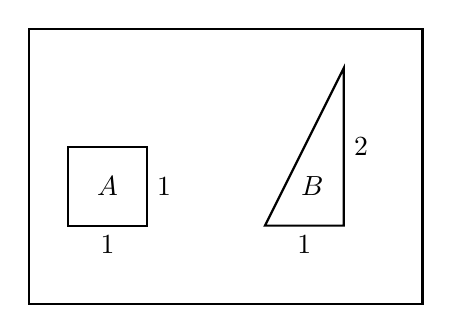
\begin{tikzpicture}[thick]
    \draw (0,0) rectangle (5,3.5);
    \draw (0.5,1) --node[below]{1}
    ++(1,0) -- node[right]{1}
    ++(0,1) -- ++(-1,0) -- cycle;
    \draw (3,1) -- node[below]{1}
    ++ (1,0)--node[right]{2}
    ++ (0,2) -- cycle;
    \draw (1,1.5)node{$A$} (3.6,1.5)node{$B$};
  \end{tikzpicture}
  \caption{落在度量相同的子区域内的等可能性.}
  \label{fig1.2.1}
  \end{minipage}%
  \begin{minipage}[b]{0.5\linewidth}
  \centering
  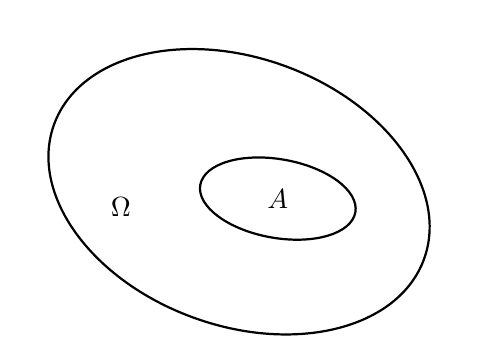
\begin{tikzpicture}[thick]
    \draw[rotate=-20] ellipse (2.5 and 1.7);
    \draw[rotate=-10,xshift=0.5cm] (0,0)node{$A$}
       ellipse (1 and 0.5);
    \node at (-1.5,-0.2) {$\Omega$};
  \end{tikzpicture}
  \caption{几何概率.}
  \label{fig1.2.2}
  \end{minipage}
\end{figure}

这个概率称为几何概率,
它满足概率的公理化定义.

求几何概率的关键是对样本空间 $\Omega$ 和所求事件 $A$ 用图形描述清楚 (一般用平面或空间图形).
然后计算出相关图形的度量 (一般为面积或体积).

\begin{example}[会商问题]
  甲乙两人约定在下午6时到7时之间在某处会面,
  并约定先到者应等候另一个人 \SI{20}{\minute},
  过时即可离去.
  求两人能会面的概率.
\end{example}

\begin{solution}
  以 $x$ 和 $y$ 分别表示甲、乙两人到达约会地点的时间 (以 \si{\minute} 为单位),
  在平面上建立 $xOy$ 直角坐标系 (见图~\ref{fig1.2.3}).

  \begin{figure}[!ht]
    \centering
    \begin{tikzpicture}[thick,>=Stealth]
    \draw[->] (-0.5,0) -- (0,0) node[below left]{$O$} -- (1,0) node[below]{20}
    -- (3,0)node[below]{60} -- (3.5,0)node[below]{$x$};
    \draw [->] (0,-0.5) -- (0,1) node[left]{20}
    -- (0,3) node[left]{60}
    -- (0,3.5) node[right] {$y$};
    \filldraw[pattern=vertical lines]
    (0,0) -- (1,0) -- (3,2) -- (3,3) --
    (2,3) -- (0,1) -- cycle;
    \draw (3,0) -- (3,2) (0,3) -- (2,3);
  \end{tikzpicture}
    \caption{会面问题中的 $\Omega$ 与 $A$.}
    \label{fig1.2.3}
  \end{figure}

  因为甲、乙都是在 0 至 \SI{60}{\minute} 内等可能地到达,
  所以由等可能性知这是一个几何概率问题.
  $(x, y)$ 的所有可能取值是边长为 60 的正方形,
  其面积为 $S_\Omega = 60^2$.
  而事件 $A =$“两人能够会面”相当于:
  \[
    | x - y | \le 20,
  \]
  即图中的阴影部分,
  其面积为 $S_A = 60^2 - 40^2$,
  由 \eqref{eq1.2.13} 式知
  \[
    P (A) = \frac{S_A}{S_\Omega} = \frac{60^2 - 40^2}{60^2} = 0.5556.
  \]
  结果表明:
  按此规则约会,
  两人能会面的概率不超过 0.6.
  若把约定时间改为在下午6时到6时30分,
  其他不变,
  则两人能会面的概率提高到 \num{0.8889}.
\end{solution}

\begin{example}[蒲丰投针问题]
  平面上画有间隔为 $d (d > 0)$ 的等距平行线,
  向平面任意投掷一枚长为 $l (l<d)$ 的针,
  求针与任一平行线相交的概率.
\end{example}

\begin{solution}
  以 $x$ 表示针的中点与最近一条平行线的距离,
  又以 $\varphi$ 表示针与此直线间的交角,
  见图~\ref{fig1.2.4}.
  易知样本空间 $\Omega$ 满足
  \[
    0 \le x \le d/2, \quad 0 \le \varphi \le \pi,
  \]
  由这两式可以确定 $x - \varphi$ 平面上的一个矩形 $\Omega$,
  这就是样本空间,
  其面积为 $S_\Omega = d\pi/2$.
  这时为了针与平行线相交 (记为事件 $A$),
  其充要条件是
  \[
    x \le \frac{l}{2} \sin \varphi.
  \]
  由这个不等式表示的区域是图~\ref{fig1.2.5} 中的阴影部分.

  由于针是向平面任意投掷的,
  所以由等可能性知这是一个几何概率问题.
  由此得
  \[
    P (A) = \frac{S_A}{S_\Omega}
    = \frac{\int_0^\pi \frac{l}{2} \sin \varphi \, \mathrm{d} \varphi}{\frac{d}{2} \pi}
    = \frac{2l}{d\pi}.
  \]

  如果 $l$, $d$ 为已知,
  则以 $\pi$ 的值代入上式即可计算得 $P(A)$ 之值.
  反之,
  如果已知 $P(A)$ 的值,
  则也可以利用上式去求 $\pi$,
  而关于 $P(A)$ 的值,
  可用从试验中获得的频率去近似它:
  即投针 $N$ 次,
  其中针与平行线相交 $n$ 次,
  则频率 $n/N$ 可作为 $P(A)$ 的估计值,
  于是由
  \[
    \frac{n}{N} \approx P (A) = \frac{2l}{d\pi},
  \]
  可得
  \[
    \pi \approx \frac{2lN}{dn}.
  \]

  历史上有一些学者曾亲自做过这个试验,
  下表记录了他们的试验结果.

  \begin{tabularx}{0.9\linewidth}{*{6}{Z}}
    \toprule
    试验者 & 年份 & $l/d$ & 投掷次数 & 相交次数 & $\pi$ 的近似值\\
    \midrule
    Wolf & 1850 & 0.8 & 5000 & 2532 & 3.1596\\
    Fox & 1884 & 0.75 & 1030 & 489 & 3.1595\\
    Lazzerini & 1901 & 0.83 & 3408 & 1808 & 3.1415\\
    Reina & 1925 & 0.54 & 2520 & 859 & 3.1795\\
    \bottomrule
  \end{tabularx}

  这是一个颇为奇妙的方法:
  只要设计一个随机试验,
  使一个事件的概率与某个未知数有关,
  然后通过重复试验,
  以频率估计概率,
  即可求得未知数的近似解.
  一般来说,
  试验次数越多,
  则求得的近似解就越精确。
  随着电子计算机的出现,
  入们便可利用计算机来大量重复地模拟所设计的随机试验。
  这种方法得到了迅速的发展和广泛的应用。
  入们称这种方法为\textbf{随机模拟法},
  也称为\textbf{蒙特卡罗 (Montecarlo) 法}.
\end{solution}

\begin{figure}
  \centering
  \begin{minipage}[b]{0.5\linewidth}
  \centering
  \begin{tikzpicture}[thick,>=Stealth,scale=1.2]
    \draw (-0.3,1) -- (4,1) (-0.3,-1)--(4,-1)
    node[below]{\phantom{$O$}};
    \draw[<->] (0,1) -- (0,-1)node[midway,fill=white]{$d$};
    \draw (2,1) -- +(45:0.3) --+ (-135:1.7);
    \draw (1.8,1) arc (180:225:0.2);
    \draw (1.51,1) --node[left]{$x$} ++(0,-0.49);
    \node at (1.7,0.85){$\varphi$};
  \end{tikzpicture}
   \caption{蒲丰投针问题}.
    \label{fig1.2.4}
  \end{minipage}%
  \begin{minipage}[b]{0.5\linewidth}
  \centering
  \begin{tikzpicture}[thick,>=Stealth]
    \draw[->](-0.3,0) -- (0,0)node[below]{$O$}
    -- (pi,0)node[below]{$\pi$} -- (4.2,0) node[below]{$\varphi$};
    \draw[->](0,0) -- (0,2.2)node[left]{$d/2$}
     -- (0,3) node[right]{$x$};
    \draw (0,2.2)--(pi,2.2)node[above right]{$\Omega$} -- (pi,0);
    \filldraw[pattern=north east lines]
    (0,0)-- plot[domain=0:pi,samples=100](\x,{1.3*sin(\x r)}) -- (pi,0)--cycle;
    \node at (1.57,1.6){$\frac l2\sin\varphi$};
  \end{tikzpicture}
  \caption{蒲丰投针问题中的 $\Omega$ 和 $A$}.
    \label{fig1.2.5}
  \end{minipage}
\end{figure}

\begin{example}
  在长度为 $a$ 的线段内任取两点将其分为三段,
  求它们可以构成一个三角形的概率.
\end{example}

\begin{solution}
  由于是将线段任意分成三段,
  所以由等可能性知这是一个几何概率问题.
  分别用 $x$, $y$ 和 $a - x - y$ 表示线段被分成的三段长度,
  见图~\ref{fig1.2.6}.
  则显然应该有
  \[
    0 < x < a; \quad 0 < y < a; \quad 0 < a - (x + y) < a.
  \]
  第三个式子等价于:
  $0 < x + y < a$.
  所以样本空间为 (见图~\ref{fig1.2.7})
  \[
    \Omega = \{(x, y): 0 < x < a, 0 < y < a, 0 < x + y < a\}.
  \]
  $\Omega$ 的面积为
  \[
    S _\Omega = \frac{a^2}{2}.
  \]

  又根据构成三角形的条件:
  三角形中任意两边之和大于第三边,
  得事件 $A$ 所含样本点 $(x,y)$ 必须满足:
  \begin{align*}
    & 0 < a - (x + y) < x + y,\\
    & 0 < x < y + (a - x - y),\\
    & 0 < y < x + (a - x - y).
  \end{align*}
  整理得
  \[
    \frac{a}{2} < x + y < a;\quad 0 < x < \frac{a}{2}; \quad 0 < y < \frac{a}{2}.
  \]
  所以事件 $A$ 可用图~\ref{fig1.2.8} 中的阴影部分表示.
  事件 $A$ 的面积为
  \[ S _A = \frac{a^2}{8}. \]
  由此得
  \[P (A) = \frac{1}{4}. \]
\end{solution}

\begin{figure}
  \begin{minipage}[b]{0.45\linewidth}
    \centering
    \begin{tikzpicture}[thick,>=Stealth,xscale=1.2]
    \draw (0,0) -- (4,0);
    \draw [densely dashed,yshift=-0.5cm](0,0) -- (4,0) node[midway,fill=white]{$a$};
    \foreach \x in {0,1,2.4,4}
      \draw(\x,-0.1) -- (\x,0.1);
    \draw[yshift=-0.5cm](0,-0.1)--(0,0.1)
    (4,-0.1)--(4,0.1);
    \draw (0.5,0.2)node{$x$} (1.7,0.2)node{$y$}
      (3.2,0.2)node{$a-x-y$};
  \end{tikzpicture}
    \caption{长度为 $a$ 的线段分成三段.}
    \label{fig1.2.6}
  \end{minipage}
  \begin{minipage}[b]{0.45\linewidth}
    \centering
    \begin{tikzpicture}[thick,>=Stealth,scale=2.6]
    \draw[->] (-0.2,0) --(1,0)node[below]{$a$}-- (1.5,0)node[below]{$x$};
    \draw[->] (0,-0.2) --(0,0)node[below left]{$O$}
    --(0,1)node[left]{$a$} -- (0,1.2)node[left]{$y$};
    \filldraw[pattern=horizontal lines] (0,0)--(1,0)
    --(0,1)--cycle;
  \end{tikzpicture}
    \caption{线段分成三段的样本空间 $\Omega$.}
    \label{fig1.2.7}
  \end{minipage}
\end{figure}

\begin{figure}
  \centering
  \begin{tikzpicture}[thick,>=Stealth,scale=2.6]
    \draw[->] (-0.2,0) --(1,0)node[below]{$a$}-- (1.5,0)node[below]{$x$};
    \draw[->] (0,-0.2) --(0,0)node[below left]{$O$}
    --(0,1)node[left]{$a$}--(0,1.2)node[left]{$y$};
    \draw (0,1) -- (1,0);
    \filldraw[pattern=horizontal lines]
    (0.5,0)node[below]{$1/2$} -- (0.5,0.5)
    --(0,0.5)node[left]{$1/2$} -- cycle;
  \end{tikzpicture}
  \caption{构成三角形的条件}
  \label{fig1.2.8}
\end{figure}

\subsection{确定概率的主观方法}

在现实世界里有一些随机现象是不能重复的或不能大量重复的,
这时有关事件的概率如何确定呢?

统计界的贝叶斯学派认为:
\textbf{一个事件的概率是人们根据经验对该事件发生的可能性所给出的个人信念}.
这样给出的概率称为\text{主观概率}.

这种利用经验确定随机享件发生可能性大小的例子是很多的,
人们也常依据某些主观概率来行事.

\begin{example}
  用主观方法确定概率的例子.
  \begin{enumerate}
    \item 在气象预报中,
    往往会说:“明天下雨的概率为 \SI{90}{\percent}”,
    这是气象专家根据气象专业知识和最近的气象情况给出的主观概率.
    听到这一信息的人,
    大多出门会带伞.

    \item 一个企业家根据他多年的经验和当时的一些市场信息,
    认为“某项新产品在未来市场上畅销”的可能性为 \SI{80}{\percent}.

    \item 一个外科医生根据自已多年的临床经验和一位患者的病情,
    认为“此手术成功”的可能性为 \SI{90}{\percent}.

    \item 一个教师根据自己多年的教学经验和甲、乙两学生的学习情况,
    认为“甲学生能考取大学”的可能性为 \SI{95}{\percent},
    “乙学生能考取大学”的可能性为 \SI{40}{\percent}.
  \end{enumerate}
\end{example}

从以上例子可以看出:
\begin{enumerate}
  \item 主观概率和主观臆造有着本质上的不同,
  前者要求当事人对所考察的事件有透彻的了解和丰富的经验,
  甚至是这一行的专家,
  并能对历史信息和当时信息进行仔细分析,
  如此确定的主观概率是可信的.
  从某种意义上说,
  不利用这些丰富的经验也是一种浪费.
  \item 用主观方法得出的随机事件发生的可能性大小,
  本质上是对随机事件概率的一种推断和估计.
  虽然结论的精确性有待实践的检验和修正,
  但结论的可信性在统计意义上是有其价值的.
  \item 在遇到的随机现象无法大量重复时,
  用主观方法去做决策和判断是适合的.
  从这点看,
  主观方法至少是频率方法的一种补充.
\end{enumerate}

另外要说明的是,
主观概率的确定除根据自己的经验外,
决策者还可以利用别人的经验。
例如,
对一项有风险的投资,
决策者向某位专家咨询的结果为“成功的可能性为 \SI{60}{\percent}”,
而决策者很熟悉这位专家,
认为专家的估计往往是偏保守的、过分蘧慎的.
为此决策者将结论修改为“成功的可能性为 \SI{70}{\percent}”.

主观给定的概率要符合公理化的定义.

\begin{xiti}
  \item 对于组合数 $\binom{n}{r}$, 证明
  \begin{enumerate}
    \item $\binom{n}{r} = \binom{n}{n - r}$;
    \item $\binom{n}{r} = \binom{n - 1}{r - 1} + \binom{n - 1}{r}$;
    \item $\binom{n}{0} + \binom{n}{1} + \dotsb + \binom{n}{n} = 2^n$;
    \item $\binom{n}{1} + 2\binom{n}{2} + \dotsb + n\binom{n}{n} = n 2^{n-1}$;
    \item $\binom{a}{0} \binom{b}{n} + \binom{a}{1} \binom{b}{n - 1} + \dotsb + \binom{a}{n} \binom{b}{0} = \binom{a + b}{n}$, $n = \min(a,b)$;
    \item $\binom{n}{0} ^2 + \binom{n}{1} ^2 + \dotsb + \binom{n}{n} ^2 = \binom{2n}{n}$.
  \end{enumerate}

  \item 抛两枚硬币,
  求至少出现一个正面的概率.

  \item 任取两个正整数,
  求它们的和为偶数的概率.

  \item 掷两颗骰子,
  求下列事件的概率:
  \begin{enumerate}
    \item 点数之和为7;
    \item 点数之和不超过5;
    \item 两个点数中一个恰是另一个的两倍.
  \end{enumerate}

  \item 考虑一元二次方程 $x^2 + Bx + C = 0$,
  其中 $B$, $C$ 分别是将一枚骰子接连掷两次先后出现的点数,
  求该方程有实根的概率 $p$ 和有重根的概率 $q$.

  \item 从一副52张的扑克牌中任取4张,
  求下列事件的概率:
  \begin{enumerate}
    \item 全是黑桃;
    \item 同花;
    \item 没有两张同一花色;
    \item 同色.
  \end{enumerate}

  \item 设5个产品中有3个合格品、2个不合格品.
  从中不返回地任取2个,
  求取出的2个中全是合格品、仅有一个合格品和没有合格品的概率各为多少?

  \item 口袋中有5个白球、3个黑球,
  从中任取两个,
  求取到的两个球颜色相同的概率.

  \item 甲口袋有5个白球、3个黑球,
  乙口袋有4个白球、6个黑球.
  从两个口袋中各任取一球,
  求取到射两个球颜色相同的概率.

  \item 从 $n$ 个数 $1, 2, \cdots, n$ 中任取2个,
  问其中一个小于 $k (1 < k < n)$,
  另一个大于 $k$ 的概率是多少?

  \item 口袋中有 10 只球,
  分别标有号码 1 到 10,
  从中不返回地任取 3 只,
  记下取出球的号码,
  试求:
  \begin{enumerate}
    \item 最小号码为5的概率;
    \item 最大号码为5的概率.
  \end{enumerate}

  \item 掷三颗骰子,
  求以下事件的概率:
  \begin{enumerate}
    \item 所得的最大点数小于等于5;
    \item 所得的最大点数等于5.
  \end{enumerate}

  \item 把10本书任意地放在书架上,
  求其中指定的三本书放在一起的概率.

  \item $n$ 个人隨机地圄一圆桌而坐,
  求甲、乙两人相邻而坐的概率.

  \item 5个人在第一层进入十一层楼的电梯.
  假如每个人以相同的概率走出任一层 (从第二层开),
  求此5个人在不同楼层走出的概率.

  \item 一个人把六根草紧在手中,
  仅露出它们的头和尾,
  然后随机地把六个头两两相接,
  六个尾也两两相接.
  求放开手后六根草恰巧连成一个环的概率.

  \item 把 $n$ 个“0”与 $n$ 个“1”随机地排列,
  求没有两个“1”连在一起的概率.

  \item 口袋中有 $n$ 个白球,
  $n$ 个黑球,
  从中一个一个不返回地摸球,
  直至摸完为止.
  求黑白球恰好相间取出的概率.

  \item $n$ 个男孩,
  $m$ 个女孩 ($m \le n + 1$) 随机地排成一排,
  试求任意两个女孩都不相邻的概率.

  \item 将3个球随机地放入4个杯子中去,
  求杯子中球的最大个数分别为1, 2, 3的概率各为多少?

  \item 将12只球随意地放人3个盒子中,
  试求第一个盒子中有3只球的概率.

  \item 将 $n$ 个完全相同的球 (这时也称球是不可辨的) 随机地放入 $N$ 个盒子中,
  试求:
  \begin{enumerate}
    \item 某个指定的盒子中恰好有 $k$ 个球的概率;
    \item 恰好有 $m$ 个空盒的概率;
    \item 某个指定的 $m$ 个盒子中恰好有 $j$ 个球的概率.
  \end{enumerate}

  \item 在区间 $(0,1)$ 中随机地取两个数,
  求事件“两数之和小于6/5”的概率.

  \item 甲乙两艘轮船驶向一个不能同时停泊两艘轮船的码头,
  它们在一昼夜内到达的时间是等可能的.
  如果甲船的停泊时间是一小时,
  乙船的停泊时间是两小时,
  求它们中任何一般都不需要等候码头空出的概率是多少?

  \item 在平面上画有间隔为 $d$ 的等距平行线,
  向平面任意投掷一个边长为 $a$, $b$, $c$ (均小于 $d$) 的三角形,
  求三角形与平行线相交的概率.

  \item 在半径为 $R$ 的圆内画平行弦,
  如果这些弦与垂直于弦的直径的交点在该直径上的位量是等可能的,
  即交点在直径上一个区间内的可能性与这区间的长度成比例,
  求任意弦的长度大于 $R$ 的概率.

  \item 设一个质点落在 $xOy$ 平面上由 $x$ 轴 $y$ 轴及直线 $x + y = 1$ 所围成的三角形内,
  而落在这三角形内各点处的可能性相等,
  即落在这三角形内任何区域上的概率与这区域的面积成正比,
  试求此质点落在直线 $x = 1/3$ 的左边的概率是多少?

  \item 设 $a > 0$,
  有任意两数 $x$, $y$,
  且 $0 < x < a$, $0 < y < a$,
  试求 $xy < a^2 / 4$ 的概率.

  \item 用主观方法确定:
  大学生中戴眼镜的概率是多少?

  \item 用主观方法确定:
  学生中考试作弊的概率是多少?
\end{xiti}

\section{概率的性质}
利用概率的公理化定义 (非负性、正则性和可列可加性),
可以导出概率的一系列性质.
以下我们逐个给出概率的一些常用性质.

首先,
在概率的正则性中说明了必然事件 $\Omega$ 的概率为1.
那么可想而知,
不可能事件 $\emptyset$ 的概率应该为0,
下面性质正说明了这一点.

\begin{property}
  \[
    P (\emptyset) = 0.
  \]
\end{property}

\begin{proof}
  由于可列个不可能事件之并仍是不可能事件,
  所以
  \[
    \Omega = \Omega \cup \emptyset \cup \emptyset \dotsb \cup \emptyset \cup \dotsb.
  \]
  因为不可能事件与任何事件是互不相容的,
  故由可列可邡性公理得
  \[
    P (\Omega) = P (\Omega) + P (\emptyset) + \dotsb + P (\emptyset) + \dotsb.
  \]
  从而由 $P (\Omega) = 1$ 得
  \[
    P (\Omega) + P (\emptyset) + \dotsb = 0.
  \]
  再由非负性公理,
  必有
  \[
    P (\emptyset) = 0.
  \]
  结论得证.
\end{proof}

\subsection{概率的可加性}

概率的可列可加性说明了对可列个互不相容的事件 $A_1$, $A_2$, $\dotsc$,
其可列并的概率可以分别求之再相加,
那么对有限个互不相容的事件 $A_1$, $A_2$, $\dotsc$, $A_n$,
其有限并的概率是否也可以分别求之再相加呢?
下面性质回答了这个问题.

\begin{property}[有限可加性]\label{prop1.3.2}
  若有限个事件 $A_1$, $A_2$, $\dotsc$, $A_n$ 互不相容,
  则有
  \begin{equation}
    P \biggl( \bigcup _{i=1} ^n A_i \biggr) = \sum_{i=1}^n P (A_i).
    \label{eq1.3.1}
  \end{equation}
\end{property}

\begin{proof}
  对 $A_1$, $A_2$, $\dotsc$, $A_n$, $\emptyset$, $\emptyset$, $\dotsc$,
  应用可列可加性,
  得
  \begin{align*}
    P \biggl( A_1\cup A_2 \cup \cdots \cup A_n \biggr)
    &= \biggl(  A_1\cup A_2 \cup \cdots \cup A_n \cup \emptyset \cup \emptyset \cup \cdots\biggr)\\
    &= P(A_1) + \cdots + P(A_n) + P (\emptyset) + P(\emptyset) + \cdots\\
    &= P(A_1) + \cdots + P(A_n).
  \end{align*}
  结论得证.
\end{proof}

由有限可加性,
我们就可以得到以下求对立事件概率的公式.

\begin{property}\label{prop1.3.3}
  对任一事件 $A$,
  有
  \begin{equation}
    P (\overline{A}) = 1 - P (A).
    \label{eq1.3.2}
  \end{equation}
\end{property}

\begin{proof}
  因为 $A$ 与 $\overline{A}$ 互不相容,
  且 $\Omega = A \cup \overline{A}$.
  所以由概率的正则性和有限可加性得 $1 = P(A) + P(\overline{A})$.
  由此得 $P(A) = 1 - P(\overline{A})$.
\end{proof}

有些事件直接考虑较为复杂,
而考虑其对立事件则相对比较简单.
对此类问题就可以利用性质~\ref{prop1.3.3},
见下面例子.

\begin{example}
  36只灯泡中4只是 \SI{60}{\watt},
  其余都是 \SI{40}{\watt} 的.
  现从中任取3只,
  求至少取到一只 \SI{60}{\watt} 灯泡的概率.
\end{example}

\begin{solution}
  记事件 $A$ 为“取出的3只中至少有一只 \SI{60}{\watt}”,
  则 $A$ 包括三种情况:
  取到一只 \SI{60}{\watt} 两只 \SI{40}{\watt},
  或取到两只 \SI{60}{\watt} 一只 \SI{40}{\watt},
  或取到三只 \SI{60}{\watt}.
  而 $A$ 的对立事件 $\overline{A}$ 只包括一种情况,
  即“取出的3只全部是 \SI{40}{\watt}”,
  由例~\ref{exmp1.2.3} 抽样模型可知
  \[
    P(\overline{A}) = \frac{\binom{32}{3}}{\binom{36}{3}}
    = \frac{248}{357} = 0.695.
  \]
  所以
  \[
    P(A) = 1 - P(\overline{A}) = \frac{109}{357} = 0.305.
  \]
\end{solution}

\begin{example}
  抛一枚硬币5次,
  求既出现正面又出现反面的概率.
\end{example}

\begin{solution}
  记事件 $A$ 为“抛5次硬币中既出现正面又出现反面”,
  则 $A$ 的情况较复杂,
  因为出现正面的次数可以是1次至4次,
  而 $A$ 的对立事件则相对简单:
  5次全部是正面 (记为 $B$),
  或5次全部是反面 (记为 $C$),
  即 $A = B \cup C$,
  其中 $B$ 与 $C$ 互不相容.
  所以由对立事件公式和概率的有限可加性得
  \begin{align*}
    P (A) &= 1 - P (\overline{A}) = 1 - P (B \cup C) = 1 - P (B) - P (C)\\
    &= 1 - \frac{1}{2^5} - \frac{1}{2^5} = \frac{15}{16}.
  \end{align*}
\end{solution}

\subsection{概率的单调性}

可以想象:
当 $B$ 被 $A$ 包含时 (即 $B$ 发生必然导致 $A$ 发生),
说明事件 $A$ 比事件 $B$ 更容易发生,
那么 $B$ 的概率不应该比 $A$ 的概率大,
这可由以下性质~\label{property1.3.4} 的推论说明之.

性质~\label{property1.3.4} 给出了两个有包含关系事件差的概率公式,
而性质~\label{property1.3.5} 给出了任意两个事件差的概率公式.

\begin{property}\label{property1.3.4}
  若 $A \supset B$,
  则
  \begin{equation}
    P (A - B) = P (A) - P (B).
    \label{eq1.3.3}
  \end{equation}
\end{property}

\begin{proof}
  因为 $A \supset B$,
  所以
  \[
    P (A - B) = B \cup (A - B),
  \]
  且 $B$ 与 $A - B$ 互不相容,
  由有限可加性得
  \[
    P (A) = P (B) + P (A - B),
  \]
  即得
  \[
    P (A - B) = P (A) - P (B).
  \]
  结论得证.
\end{proof}

\begin{corollary}{}
  若 $A \supset B$,
  则 $P (A) \ge P (B)$.
\end{corollary}

很容易举例说明:
以上推论的逆命题不成立,
即由 $P (A) \ge P (B)$ 无法推出 $A \supset B$.

\begin{property}\label{property1.3.5}
  对任意两个事件 $A$, $B$, 有
  \begin{equation}
    P (A - B) = P (A) - P (AB).
    \label{eq1.3.4}
  \end{equation}
\end{property}

\begin{proof}
  因为 $A - B = A - AB$,
  且 $AB \subset A$,
  所以由性质~\label{property1.3.4} 得
  \[
     p (A - B) = P (A - AB) = P (A) - P (AB).
  \]
  结论得证.
\end{proof}

利用性质~\label{property1.3.4},
我们可以求一些较为复杂的事件的概率.

\begin{example}
  口袋中有编号为 1, 2, \dots, $n$ 的 $n$ 个球,
  从中有放回地任取 $m$ 次,
  求取出的 $m$ 个球的最大号码为 $k$ 的概率.
\end{example}

\begin{solution}
  记事件 $A_k$ 为“取出的 $m$ 个球的最大号码为 $k$”.
  如果直接考虑事件 $A_k$,
  则比较复杂,
  因为“最大号码为 $k$”可以包括取到1次 $k$、取到2次 $k$、\dots、取到 $m$ 次$k$.

  为此我们记事件 $B_i$ 为“取出的 $m$ 个球的最大号码小于等于 $i$”, $i=1$, $2$, $\dotsc$, $n$.
  则 $B$ 发生只需每次从 $1$, $2$, $\dotsc$, $i$ 号球中取球即可.
  所以由古典概率知
  \[
    P(B_i) = \frac{i^m}{n^m}, \quad i = 1, 2, \dotsc, n.
  \]
  又因为 $A_k = B_k - B_{k-1}$,
  且 $B_{k-1} \subset B_k$,
  由性质~\label{property1.3.4} 得
  \begin{align*}
    P(A_k) &= P(B_k - B_{k-1}) = P(B_k) - P(B_{k-1})\\
    &= \frac{k^m - (k - 1)^m}{n^m}, \quad k = 1,2, \dotsc, n.
  \end{align*}

  譬如,
  $n = 6$, $m = 3$,
  可算得
  \[
    P(A_4) = \frac{4^3 - 3^3}{6^3} = \frac{37}{216} = 0.1713.
  \]
  其他的 $P(A_k)$ 也都可算出,
  现列表如下:

  \begin{tabularx}{\linewidth}{*{8}{Z}}
    \toprule
    $k$ & 1 & 2 & 3 & 4 & 5 & 6 & 和\\
    \midrule
    $P(A_k)$ & 0.0046 & 0.0324 & 0.0880 & 0.1713 & 0.2824 & 0.4213 & 1.000\\
    \bottomrule
  \end{tabularx}

  这相当于掷三颗骰子,
  最大点数为6的概率是0.4213,
  而由
  \[
    P(k \le 3) = 0.0046 + 0.0324 + 0.0880 = 0.1250.
  \]
  说明:
  掷三颗骰子,
  最大点数不超过3的概率仅为0.1250.
\end{solution}

\subsection{概率的加法公式}

当事件之间互不相容时,
有限可加性或可列可加性给出了求事件并的概率的公式。
那么对一般的事件 (不一定互不相容),
又如何求事件并的概率?
以下性质~\label{property1.3.6} 给出求任意两个事件并的概率加法公式,
\eqref{eq1.3.6} 给出求任意 $n$ 个事件并的概率加法公式.
这些性质在计算概率时是非常有用的.

\begin{property}[加法公式]\label{property1.3.6}
  对任意两个事件 $A$, $B$, 有
  \begin{equation}
    P(A \cup B) = P(A) + P(B) - P(AB).
    \label{eq1.3.5}
  \end{equation}
  对任意 $n$ 个事件 $A_1$, $A_2$, $\dotsc$, $A_n$, 有
  \begin{multline}
    P \biggl( \bigcup_{i=1}^n A_i \biggr) = \sum_{i=1}^n P (A_i)
    - \sum_{1 \le i < j < \le n} P(A_i A_j)
    + \sum_{1 \le i < j < k \le n} P(A_i A_j A_k)\\
    + \dotsb + (-1)^{n-1} P(A_1 A_2 \dotsb A_n).
    \label{eq1.3.6}
  \end{multline}
\end{property}

\begin{proof}
  先证 \eqref{eq1.3.5}. 因为
  \[
    A \cup B = A \cup (B - A),
  \]
  且 $A$ 与 $B - A$ 互不相容,
  所以由有限可加性和性质~\label{property1.3.5}得
  \[
    P (A \cup B) = P (A) + P (B - A) = P (A) + P (B) - P(AB).
  \]

  下面用归纳法证明 \eqref{eq1.3.6}.
  当 $n=2$ 时,
  \eqref{eq1.3.6} 即为 \eqref{eq1.3.5}.
  设 \eqref{eq1.3.6} 对 $n - 1$ 成立,
  则对 $n$,
  先对两个事件 $(A_1 \cup A_2 \cup \dotsb \cup A_{n-1})$ 与 $A_n$ 用 \eqref{eq1.3.5},
  \begin{align*}
    P (A_1 \cup A_2 \cup \dotsb \cup A_n)
    &= P (A_1 \cup A_2 \cup \dotsb \cup A_{n-1}) + P (A_n)
    - P ( (A_1 \cup A_2 \cup \dotsb \cup A_{n-1}) \cap A_n )\\
    &= P (A_1 \cup A_2 \cup \dotsb \cup A_{n-1}) + P (A_n)
    - P ( (A_1 A_n) \cup (A_2 A_n) \cup \dotsb \cup (A_{n-1} A_n) ).
  \end{align*}
  然后由归纳假设,
  对
  \[
    P (A_1 \cup A_2 \cup \dotsb \cup A_{n-1})
    \quad \text{及} \quad
    P ( (A_1 A_n) \cup (A_2 A_n) \cup \dotsb \cup (A_{n-1} A_n) )
  \]
  进行展开,
  经过整理合并即可知:
  \eqref{eq1.3.6} 对 $n$ 也成立,
  结论得证.
\end{proof}

\begin{corollary}{半可加性}
  对任意两个事件 $A$, $B$,
  有
  \begin{equation}
    P (A \cup B) \le P (A) + P (B).
    \label{eq1.3.7}
  \end{equation}
  对任意 $n$ 个事件 $A_1$, $A_2$, $\dotsc$, $A_n$,
  有
  \begin{equation}
    P \biggl( \bigcup _{i=1} ^n A_i \biggr) \le \sum _{i=1} ^n P (A_i).
    \label{eq1.3.8}
  \end{equation}
\end{corollary}

\begin{example}
  已知事件 $A$, $B$, $A \cup B$ 的概率分别为 0.4, 0.3, 0.6,
  求 $P (A \overline{B})$.
\end{example}

\begin{solution}
  由加法公式及题没条件知:
  \[
    0.6 = 0.4 + 0.3 - P (AB),
  \]
  由此解得 $P (AB) = 0.1$,
  所以再由 \eqref{eq1.3.4} 得
  \[
    P (A \overline{B}) = P (A - B) = P (A) - P (AB) = 0.4 - 0.1 = 0.3.
  \]
\end{solution}

\begin{example}
  已知 $P (A) = P (B) = P (C) = 1/4$,
  $P (AB) = 0$,
  $P (AC) = P (BC) = 1/16$.
  则 $A$, $B$ ,$C$ 中至少发生一个的概率是多少?
  $A$, $B$, $C$ 都不发生的概率是多少?
\end{example}

\begin{solution}
  因为 $P (AB) = 0$,
  且 $ABC \subset AB$,
  所以由概率的单调性知 $P (ABC) = 0$.
  再由加法公式,
  得 $A$, $B$, $C$ 中至少发生一个的概率为
  \begin{align*}
    P (A \cup B \cup C)
    &= P (A) + P (B) + P (C) - P (AB) - P (AC) - P (BC) + P (ABC)\\
    &= \frac{3}{4} - \frac{2}{16} = \frac{5}{8}.
  \end{align*}

  又因为“$A$, $B$, $C$ 都不发生”的对立事件为“$A$, $B$, $C$ 中至少发生一个”,
  所以由对立事件公式得
  \[
    P (A, B, C \text{ 都不发生}) = 1 - \frac{5}{8} = \frac{3}{8}.
  \]
\end{solution}

一般而言,
求“至少有一个……”的概率时,
用对立事件公式去求较为方便.
但下面例~\ref{exam1.3.6} 的配对问题却不能用对立事件去求解,
而一定要将事件“至少有个……”表示成事件的并,
然后用一般事件的加法公式去求解.

\begin{example}[配对问题]\label{exam1.3.6}
  在一个有 $n$ 个人参加的晚会上,
  每个人带了一件礼物,
  且假定各人带的礼物都不相同.
  晚会期间各人从放在一起的 $n$ 件礼物中随机抽取一件,
  问至少有一个人自己抽到自己礼物的概率是多少?
\end{example}

\begin{solution}
  以 $A_i$ 记事件“第 $i$ 个人自己抽到自己的礼物”,
  $i=1,\dotsc,n$.
  所求概率为 $P(A_1 \cup A_2 \cup \dotsb \cup A_n)$.
  因为
  \begin{align*}
    & P(A_1) = P(A_2) = \dotsb = P(A_n) =\frac{1}{n},\\
    & P(A_1 A_2) = P(A_1 A_3) = \dotsb = P(A_{n-1} A_n) = \frac{1}{n (n-1)},\\
    & P(A_1 A_2 A_3) = P(A_1 A_2 A_4) = \dotsb = P(A_{n-2} A_{n-1} A_n) = \frac{1}{n (n-1) (n-2)},\\
    & \ldots\\
    & P(A_1 A_2 \dotsb A_n) = \frac{1}{n!}.
  \end{align*}
  所以由概率的加法公式 \eqref{eq1.3.6} 得
  \[
    P(A_1 \cup A_2 \cup \dotsb \cup A_n) = 1 - \frac{1}{2!} + \frac{1}{3!} - \frac{1}{4!} + \dotsb + (-1)^{n-1} \frac{1}{n!}.
  \]
  譬如,
  当 $n=5$ 时,
  此概率为 \num{0.6333};
  当 $n \ge 10$ 时,
  此概率近似为 $1 - e^{-1} = 0.6321$.
  这表明:
  即使参加晚会的人很多 (譬如 100 人以上),
  事件“至少有一个人自己抽到自己礼物”也不是必然事件.
\end{solution}

\subsection{概率的连续性}

为了讨论概率的连续性,
我们先对事件序列的极限给出如下的定义.

\begin{definition}{}{1.3.1}
  \begin{enumerate}
    \item 对 $\mathscr{F}$ 中任一单调不减的事件序列 $F_1 \subset F_2 \subset \dotsb \subset F_n \subset \dotsb$,
    称可列并 $\bigcup_{n=1}^{+\infty} F_n$ 为 $\{ F_n \}$ 的\textbf{极限事件},
    记为
    \begin{equation}
      \lim_{n \to +\infty} F_n = \bigcup_{n=1}^{+\infty} F_n.
      \label{eq1.3.9}
    \end{equation}

    \item 对 $\mathscr{F}$ 中任一单调不增的事件序列 $E_1 \supset E_2 \supset \dotsb \supset E_n \supset \dotsb$,
    称可列交 $\bigcap_{n=1}^{+\infty} E_n$ 为 $\{ E_n \}$ 的\textbf{极限事件},
    记为
    \begin{equation}
      \lim _{n \to +\infty} E _n = \bigcap _{n=1} ^{+\infty} E_n.
      \label{eq1.3.10}
    \end{equation}
  \end{enumerate}
\end{definition}

有了以上极限事件的定义,
我们就可如下给出一个概率函数的连续性定义.

\begin{definition}{}{1.3.2}
  对 $\mathscr{F}$ 上的一个概率 $P$,
  \begin{enumerate}
    \item 若它对 $\mathscr{F}$ 中任一单调不减的事件序列 $\{F_n\}$ 均成立
    \[
      \lim _{n \to +\infty} P (F_n) = P (\lim _{n \to +\infty} F_n),
    \]
    则称概率 $P$ 是\textbf{下连续}的.

    \item 若它对 $\mathscr{F}$ 中任一单调不增的事件序列 $\{E_n\}$ 均成立
    \[
      \lim _{n \to +\infty} P (E_n) = P (\lim _{n \to +\infty} E_n),
    \]
    则称概率 $P$ 是\textbf{上连续}的.
  \end{enumerate}
\end{definition}

有了以上的定义,
我们就可以证明概率的连续性了.

\begin{property}[概率的连续性]\label{prop1.3.7}
  若 $P$ 为事件域上的概率,
  则 $P$ 既是下连续的,
  又是上连续的.
\end{property}

\begin{proof}
  先证 $P$ 的下连续性.
  设 $\{F_n\}$ 是 $\mathscr{F}$ 中一个单调不减的事件序列,
  即
  \[
    \bigcup _{i=1} ^{+\infty} F_i = \lim _{n \to +\infty} F_n.
  \]
  若定义 $F_0 = \emptyset$,
  则
  \[
    \bigcup _{i=1} ^{+\infty} F_i = \bigcup _{i=1} ^{+\infty} (F_i - F_{i-1}).
  \]
  由于 $F_{i-1} \subset F_i$,
  显然诸 $(F_i, F_{i-1})$ 两两不相容,
  再由可列可加性得
  \[
    P \biggl( \bigcup _{i=1} ^{+\infty} F_i \biggr) = \sum _{i=1} ^{+\infty} P (F_i - F_{i-1}) = \lim_{n \to +\infty} \sum _{i=1} ^n P (F_i - F_{i-1}).
  \]
  又由有限可加性得
  \[
    \sum _{i=1} ^n P (F_i - F_{i-1}) = P \biggl( \bigcup _{i=1} ^n (F_i - F_{i-1}) \biggr) = P (F_n).
  \]
  所以
  \[
    P (\lim _{n \to +\infty} F_n) = \lim _{n \to +\infty} P (F_n).
  \]
  这就证得了 $P$ 的下连续性.

  再证 $P$ 的上连续性.
  设 $\{ E_n \}$ 是单调不增的事件序列,
  则 $\{ \overline{E}_n \}$ 为单调不减的事件序列,
  由概率的下连续性得
  \begin{align*}
    1 - \lim _{n \to +\infty} P (E_n)
    &= \lim _{n \to +\infty} [1 - P (E_n)] = \lim _{n \to +\infty} P (\overline{E} _n)\\
    &= P \biggl( \bigcup _{n=1} ^{+\infty} \overline{E}_n \biggr)
    = P \biggl( \overline{\bigcap _{n=1} ^{+\infty} E_n} \biggr)\\
    &= 1 - P \biggl( \bigcap _{n=1} ^{+\infty} E_n \biggr).
  \end{align*}
  注意最后第二个等式用了德莫根公式.
  至此得
  \[
    \lim _{n \to +\infty} P (E_n) = P \biggl( \bigcap _{n=1} ^{+\infty} E_n \biggr).
  \]
  这就证得了 $P$ 的上连续性.
\end{proof}

下面我们对可列可加性作进一步讨论.
从上面的讨论可知,
由可列可加性可推出有限可加性和下连续性,
但由有限可加性不能推出可列可加性.
这意味着要由有限可加性去推可列可加性,
还缺少条件.
下面性质说明:
所缺少的条件就是下连续性.

\begin{property}\label{prop1.3.8}
  若 $P$ 是 $\mathscr{F}$ 上满足 $P(\Omega) = 1$ 的非负集合函数,
  则它具有可列可加性的充要条件是 (1) 它是有限可加的; (2) 它是下连续的.
\end{property}

\begin{proof}
  必要性可从性质~\ref{prop1.3.2} 和性质~\ref{prop1.3.7} 获得.
  下证充分性.

  设 $A_i \in \mathscr{F}$, $i=1,2,\dotsc$ 是两两不相容的事件序列,
  由有限可加性可知:
  对任意有限的 $n$ 都有
  \[
    P \biggl( \bigcup _{i=1} ^n A_i \biggr) = \sum _{i=1} ^n P (A_i).
  \]
  这个等式的左边不超过1,
  因此正项级数 $\sum _{i=1} ^{+\infty} P (A_i)$ 收敛,
  即
  \begin{equation}
    \lim _{n \to +\infty} P \biggl( \bigcup _{i=1} ^n A_i \biggr)
    = \lim _{n \to +\infty} \sum _{i=1} ^n P (A_i)
    = \sum _{i=1} ^{+\infty} P (A_i).
    \label{eq1.3.11}
  \end{equation}
  记
  \[
    F_i = \bigcup _{i=1} ^n A_i,
  \]
  则 $\{Fn\}$ 为单调不减的事件序列,
  所以由下连续性得
  \begin{equation}
    \lim _{n \to +\infty} P \biggl( \bigcup _{i=1} ^n A_i \biggr)
    = \lim _{n \to +\infty} P (F_n)
    = P \biggl( \bigcup _{n=1} ^{+\infty} F_n \biggr)
    = P \biggl( \bigcup _{n=1} ^{+\infty} A_n \biggr).
    \label{eq1.3.12}
  \end{equation}
  综合 \eqref{eq1.3.11} 和 \eqref{eq1.3.12},
  即得可列可加性.
\end{proof}

从性质~\ref{prop1.3.8} 可以看出:
在概率的公理化定义中,
可以将可列可加性换成是有限可加性和下连续性.

\begin{xiti}
  \item 对下述五个事件发生可能性的文宇插述找出最合适的数值答案:\\
  \begin{tabularx}{0.7\linewidth}{p{0.5\linewidth}l}
    \toprule
    文字描述 & 数值答案\\
    \midrule
    (1) 事件 $A$ 发生与不发生的可能性一样 & (a) 0\\
    (2) 事件 $B$ 很可能发生, 但不一定发生 & (b) 0.1\\
    (3) 事件 $C$ 肯定不发生 & (c) 0.5\\
    (4) 事件 $D$ 能够发生, 但可能性不大 & (d) 0.9\\
    (5) 事件 $E$ 必定会发生 & (e) 1\\
    \bottomrule
  \end{tabularx}

  \item 设 $P (AB) = 0$,
  则下列说法哪些是正确的?
  \begin{enumerate}
    \item $A$ 和 $B$ 不相容;
    \item $A$ 和 $B$ 相容;
    \item $AB$ 是不可能事件;
    \item $AB$ 不一定是不可能事件;
    \item $P(A) = 0$, 或 $P(B) = 0$;
    \item $P(A-B) = P(A)$.
  \end{enumerate}

  \item 一批产品分一、二、三级,
  其中一级品是二级品的两倍,
  三级品是二级品的一半,
  从这批产品中随机地抽取一个,
  试求取到二级品的概率.

  \item 从0, 1, 2, \dots,9 等十个数字中任意选出三个不同的数字,
  试求下列事件的概率:
  \begin{enumerate}
    \item $A_1 = \{ \text{三个数字中不含 0 和 5} \}$;
    \item $A_2 = \{ \text{三个数字中不含 0 或 5} \}$;
    \item $A_3 = \{ \text{三个数字中含 0 但不含 5} \}$.
  \end{enumerate}

  \item 某城市中共发行3种报纸 A, B, C.
  在这城市的居民中有 \SI{45}{\percent} 订阅 A 报、\SI{35}{\percent} 订阅 B 报、\SI{30}{\percent} 订阅 C 报,
  \SI{10}{\percent} 同时订阅 A 报 B 报、\SI{8}{\percent} 同时订阅 A 报 C 报、\SI{5}{\percent} 同时订阅 B 报 C 报、\SI{3}{\percent} 同时订阅 A, B, C 报.
  求以下事件的百分率:
  \begin{enumerate}
    \item 只订阅 A 报的;
    \item 只订阅一种报纸的;
    \item 至少订阅一种报纸的;
    \item 不订阅任何一种报纸的.
  \end{enumerate}

  \item 某工厂一个班组共有男工7人、女工4人,
  现要选出3个代表,
  问选的3个代表中至少有1个女工的概率是多少?

  \item 赌徒认为掷一颗骰子4次至少出现一次6点与掷两颗骰子24次至少出现一次双6点的机会是相等的,
  你认为如何?

  \item 从数字1, 2, \dots, 9中可重复地任取 $n$ 次,
  求 $n$ 次所取数字的乘积能被10整除的概率.

  \item 口袋中有 $n-1$ 个黑球和 1 个白球,
  每次从口袋中随机地摸出一球,
  并换入一只黑球.
  问第 $k$ 次摸球时,
  摸到黑球的概率是多少?

  \item 甲掷硬币 $n+1$ 次,
  乙掷 $n$ 次.
  求甲掷出的正面数比乙掷出的正面数多的概率.

  \item 掷 $2n+1$ 次硬币,
  求出现的正面数多于反面数的概率.

  \item 有三个人,
  每个人都以同样的概率 $1/4$ 被分配到四个房间中的每一间中,
  试求:
  \begin{enumerate}
    \item 三个人都分配到同一个房间的概率;
    \item 三个人分配到不同房间的概率.
  \end{enumerate}

  \item 一间宿舍内住有6位同学,
  求他们之中至少有2个人的生日在同一个月份的概率.

  \item 某班 $n$ 个战士各有1支归个人保管使用的枪,
  这些枪的外形完全一样,
  在一次夜间紧急集合中,
  每人随机地取了1支枪,
  求至少有1人拿到自己的枪的概率.

  \item 设 $A$, $B$ 是两事件,
  且 $P(A) = 0.6$,
  $P(B) = 0.7$,
  问:
  \begin{enumerate}
    \item 在什么条件下 $P(AB)$ 取到最大值,
    最大值是多少?
    \item 在什么条件下 $P(AB)$ 取到最小值,
    最小值是多少?
  \end{enumerate}

  \item 已知事件 $A$, $B$ 满足 $P(AB) = P(\overline{A} \cap \overline{B})$,
  记 $P(A) = p$,
  试求 $P(B)$.

  \item 已知 $P(A) = 0.7$,
  $P(A-B) = 0.3$,
  试求 $P(\overline{AB})$.

  \item 设 $P(A) = P(B) = 1/2$,
  试证 $P(AB) = P(A \cap B)$.

  \item 对任意的事件 $A$, $B$, $C$,
  证明:
  \begin{enumerate}
    \item $P (AB) + P (AC) - P (BC) \le P (A)$,
    \item $P (AB) + P (AC) + P (BC) \ge P (A) + P (B) + P (C) - 1$.
  \end{enumerate}

  \item 设 $A$, $B$, $C$ 为三个事件,
  且 $P(A) = a$, $P(B) = 2a$, $P(C) = 3a$,
  $P(AB) = P(AC) = P(BC) = b$,
  证明:
  $a \le 1/4$, $b \le 1/4$.

  \item 设事件 $A$, $B$, $C$ 的概率都是1/2,
  且 $P(ABC) = P(\overline{A} \cap \overline{B} \cap \overline{C})$,
  证明:
  \[
    2P(ABC) = P(AB) + P(AC) + P(BC) / 1/2.
  \]

  \item 证明:
  \begin{enumerate}
    \item $P(AB) \ge P(A) + P(B) - 1$,
    \item $P(A_1 A_2 \dotsb A_n) \ge P(A_1) + P(A_2) + \dotsb + P(A_n) - (n-1)$.
  \end{enumerate}

  \item 证明:
  \[
    \lvert P(AB) - P(A)P(B) \rvert \le \frac{1}{4}.
  \]
\end{xiti}

\section{条件概率}

条件概率是概率论中的一个既重要又实用的概念。

\subsection{条件概率的定义}

所谓条件概率,
它是指在某事件 $B$ 发生的条件下,
求另一事件 $A$ 的概率,
记为 $P(A|B)$,
它与 $P(A)$ 是不同的两类概率.
下面用一个例子说明之.

\begin{example}
  考察有两个小孩的家庭,
  其样本空间为 $\Omega = \{bb,bg,gb,gg\}$,
  其中 $b$ 代表男孩,
  $g$ 代表女孩,
  $bg$ 表示大的是男孩、小的是女孩,
  其他样本点可类似说明.

  在 $\Omega$ 中4个样本点等可能情况下,
  我们来讨论如下一些事件的概率.
  \begin{enumerate}
    \item 事件 $A=$“家中至少有一个女孩”发生的概率为
    \[
      P(A) = \frac{3}{4}.
    \]

    \item 若已知事件 $B=$“家中至少有一个男孩”发生,
    再求事件 $A$ 发生的概率为
    \[
      P(A|B) = \frac{2}{3}.
    \]
    这是因为事件 $B$ 的发生,
    排除了 $gg$ 发生的可能性,
    这时样本空间 $\Omega$ 也随之改为 $\Omega_B = \{bb,bg,gb\}$,
    而在 $\Omega_B$ 中事件 $A$ 只含2个样本点,
    故 $P(A|B) = 2/3$.
    这就是条件概率,
    它与 (无条件) 概率 $P (A)$ 是不同的两个概念.

    \item 若对上述条件概率的分子分母各除以4,
    则可得
    \[
      P(A|B) = \frac{2/4}{3/4} = \frac{P(AB)}{P(B)},
    \]
    其中交事件 $AB=$“家有一男一女两个小孩”.
  \end{enumerate}
\end{example}

这个关系具有一般性,
即条件概率是两个无条件概率之商,
这就是条件概率的定义.

\begin{definition}{}{1.4.1}
  设 $A$ 与 $B$ 是样本空间 $\Omega$ 中的两事件,
  若 $P(B) > 0$,
  则称
  \begin{equation}
    P(A|B) = \frac{P(AB)}{P(B)}.
    \label{eq1.4.1}
  \end{equation}
  为“\textbf{在 $B$ 发生下 $A$ 的条件概率}”,
  简称\textbf{条件概率}.
\end{definition}

\begin{example}\label{exam1.4.2}
  设某样本空间 $\Omega$ 含有25个等可能的样本点,
  事件 $A$ 含有15个样本点,
  事件 $B$ 含有7个样本点,
  交事件 $AB$ 含有5个样本点,
  具体见图~\ref{fig1.4.1}.

  \begin{figure}
    \centering
    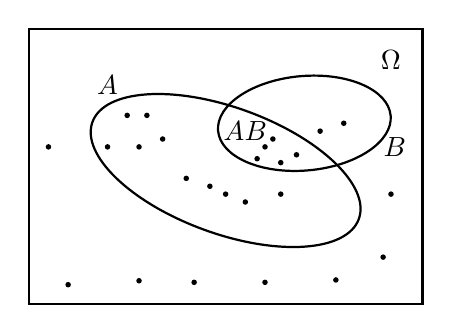
\begin{tikzpicture}[thick]
  \draw (0,0) rectangle (5,3.5);
  \draw[rotate around={-20:(2.5,1.7)}](2.5,1.7) circle (1.8 and 0.8);
  \draw[rotate around={5:(3.5,2.3)}] (3.5,2.3) ellipse (1.1 and 0.6);
  \node at (4.6,3.1) {$\Omega$};
  \node at (2.75,2.2) {$AB$};
  \node at (4.65,2) {$B$};
  \node at (1,2.78) {$A$};
  \foreach \x/\y in {
    3/2, 2.9/1.85, 3.1/2.1, 3.2/1.8, 3.4/1.9,
    3.7/2.2, 4/2.3,
    0.25/2, 0.5/0.25, 1.4/0.3, 2.1/0.28,
    3/0.28, 3.9/0.31, 4.5/0.6, 4.6/1.4,
    1/2, 1.25/2.4, 1.5/2.4, 1.7/2.1, 1.4/2,
    2/1.6, 2.3/1.5, 2.5/1.4, 2.75/1.3, 3.2/1.4
  }
  \fill(\x,\y) circle(1pt);
\end{tikzpicture}
    \caption{例~\ref{exam1.4.2} 的维恩图.}\label{fig1.4.1}
  \end{figure}

  这时有
  \begin{align*}
    & P(A) = \frac{15}{25},\\
    & P(B) = \frac{7}{25},\\
    & P(AB) = \frac{5}{25}.
  \end{align*}
  则在事件 $B$ 发生的条件下,
  事件 $A$ 的条件概率为
  \[
    P (A|B) = \frac{P(AB)}{p(B)} = \frac{5/25}{7/25} = \frac{5}{7}.
  \]

  此结果也可以如此考虑:
  事件 $B$ 发生,
  表明事件 $\overline{B}$ 不可能发生,
  因此 $\overline{B}$ 中的18个样本点可以不予考虑.
  此时在 $B$ 中7个样本点中属于 $A$ 的只有5个,
  所以 $P(A|B) = 5/7$.
  这意味着,
  在计算条件概率 $P(A|B)$ 时,
  样本空间 $\Omega$ 缩小为 $\Omega_B = B$.

  类似地
  \[
    P (B|A) = \frac{P(AB)}{P(A)} = \frac{5/25}{15/25} = \frac{1}{3}.
  \]
  它也可作如上解释.
\end{example}

我们要注意的是:
条件概率 $P(A|B)$ 是在给定 $B$ 下讨论事件 $A$ 的概率,
那么概率的性质对 $P(\cdot|B)$ 而言是否都成立呢?
譬如
\[
  P (\overline{A} | B) = 1 - P(A|B),
\]
\[
  P(A_1 \cup A_2 | B) = P(A_1 | B) + P(A_2 | B) - P(A_1 A_2 | B)
\]
这些概率性质都成立吗?
为此我们只要能验证条件概率满足三条公理即可回答这个问题.

\begin{property}
  条件概率是概率,
  即若设 $P(B) > 0$,
  则
  \begin{enumerate}
    \item $P(A|B) \ge 0$, $A \in \mathscr{F}$,
    \item $P(\Omega|B) = 1$,
    \item 若 $\mathscr{F}$ 中的 $A_1$, $A_2$,\dots,$A_n$,\dots 互不相容,
    则
    \[
      P \biggl( \bigcup _{n=1} ^{+\infty} A_n | B \biggr) = \sum_{n=1} ^{+\infty} P (A_n | B).
    \]
  \end{enumerate}
\end{property}

\begin{proof}
  用条件概率的定义很容易证明前两点.
  下面来证明第三点.
  因为 $A_1$, $A_2$, \dots, $A_n$, \dots 互不相容,
  所以 $A_1B$, $A_2B$, \dots, $A_nB$, \dots 也互不相容,
  故
  \begin{align*}
    P \biggl( \bigcup _{n=1} ^{+\infty} A_n | B \biggr)
    &= \frac{P \Biggl( \biggl( \bigcup _{n=1} ^{+\infty} A_n \biggr) B \Biggr)}{P (B)}
    = \frac{P \biggl( \bigcup _{n=1} ^{+\infty} (  A_n B ) \biggr)}{P (B)}\\
    &= \sum _{n=1} ^{+\infty} \frac{P (A_n B)}{P(B)}
    = \sum _{n=1} ^{+\infty} P (A_n | B).
  \end{align*}
\end{proof}

以下给出条件概率特有的三个非常实用的公式:
乘法公式、全概率公式和贝叶斯公式.
这些公式可以帮助我们计算一些复杂事件的概率.

\subsection{乘法公式}

\begin{property}[乘法公式]
  \begin{enumerate}
    \item 若 $P(B) > 0$,
    则
    \begin{equation}
      P(AB) = P(B) P(A|B).
      \label{eq1.4.2}
    \end{equation}
    \item 若 $P(A_1 A_2 \dotsb A_{n-1}) > 0$,
    则
    \begin{equation}
      P(A_1 \dotsb A_n) = P(A_1) P(A_2 | A_1) P(A_3 | A_2 A_1) \dotsb P(A_n | A1 \dotsb A_{n-1}).
      \label{eq1.4.3}
    \end{equation}
  \end{enumerate}
\end{property}

\begin{proof}
  由条件概率的定义,
  移项即得 \eqref{eq1.4.2}.
  下证 \eqref{eq1.4.3},
  因为
  \[
    P(A_1) \ge P(A_1 A_2) \ge \dotsb \ge P(A_1 \dotsb A_{n-1}) > 0,
  \]
  所以 \eqref{eq1.4.3} 中的条件概率均有意义,
  且按条件概率的定义,
  \eqref{eq1.4.3} 的右边等于
  \[
    P(A_1)
    \cdot \frac{P(A_1 A_2)}{P(A_1)}
    \cdot \frac{P(A_1 A_2 A_3)}{P(A_1 A_2)}
    \cdot \dotsb
    \cdot \frac{P(A_1 \dotsb A_n)}{P(A_1 \dotsb A_{n-1})}
    = P(A_1 \dotsb A_n).
  \]
  从而 \eqref{eq1.4.3} 式成立.
\end{proof}

\begin{example}\label{exam1.4.3}
  一批零件共有100个,
  其中有10个不合格品.
  从中一个一个取出,
  求第三次才取得不合格品的概率是多少?
\end{example}

\begin{solution}
  以 $A_i$ 记事件“第 $i$ 次取出的是不合格品”,
  $i=1,2,3$.
  则所求概率为 $P(\overline{A_1} \overline{A_2} A_3)$,
  由乘法公式得
  \begin{align*}
    P(\overline{A_1} \overline{A_2} A_3)
    &= P(\overline{A_1}) P(\overline{A_2} | \overline{A_1}) P(A_3 | \overline{A_1} \overline{A_2})\\
    &= \frac{90}{100} \frac{89}{99} \frac{10}{98} = 0.0826.
  \end{align*}
\end{solution}

其实,例~\ref{exam1.4.3} 是下面例~\ref{exam1.4.4} 的特例.

\begin{example}[罐子模型]\label{exam1.4.4}
  设罐中有 $b$ 个黑球、$r$ 个红球,
  每次随机取出一个球,
  取出后将原球放回,
  还加进 $c$ 个同色球和 $d$ 个异色球.
  记 $B_i$ 为“第 $i$ 次取出的是黑球”,
  $R_j$ 为“第 $j$ 次取出的是红球”.

  若连续从罐中取出三个球,
  其中有两个红球、一个黑球.
  则由乘法公式我们可得
  \begin{align*}
    P(B_1 R_2 R_3)
    &= P(B_1) P(R_2 | B_1) P(R_3 | B_1 R_2)\\
    &= \frac{b}{b+r} \frac{r+d}{b+r+c+d} \frac{r+d+c}{b+r+2c+2d},\\
    P(R_1 B_2 R_3)
    &= P(R_1) P(B_2 | R_1) P(R_3 | R_1 B_2)\\
    &= \frac{r}{b+r} \frac{b+d}{b+r+c+d} \frac{r+d+c}{b+r+2c+2d},\\
    P(R_1 R_2 B_3)
    &= P(R_1) P(R_2 | R_1) P(B_3 | R_1 R_2)\\
    &= \frac{r}{b+r} \frac{r+c}{b+r+c+d} \frac{b+2d}{b+r+2c+2d}.
  \end{align*}
  以上概率与黑球在第几次被抽取有关.
\end{example}

罐子模型也称为波利亚 (Polya) 模型,
这个模型可以有各种变化,
具体见下:

\begin{enumerate}
  \item 当 $c=-1$, $d=0$ 时,
  即为\textbf{不返回抽样}.
  此时前次抽取结果会影响后次抽取结果.
  但只要抽取的黑球与红球个数确定,
  则概率不依赖其抽出球的次序,
  都是一样的.
  此例中有
  \begin{align*}
    P(B_1 R_2 R_3) &= P(R_1 B_2 R_3) = P(R_1 R_2 B_3)\\
    &= \frac{br(r-1)}{(b+r) (b+r-1) (b+r-2)}.
  \end{align*}
  例~\ref{exam1.4.3} 可以归结为此种情况.

  \item 当 $c=0$, $d=0$ 时,
  即为\textbf{返回抽样}.
  此时前次抽取结果不会影响后次抽取结果.
  故上述三个概率相等,
  且都等于
  \[
    P(B_1 R_2 R_3) = P(R_1 B_2 R_3) = P(R_1 R_2 B_3) = \frac{br^2}{(b+r)^3}.
  \]

  \item 当 $c>0, d=0$ 时,
  称为\textbf{传染病模型}.
  此时,
  每次取出球后会增加下一次取到同色球的概率,
  或换句话说,
  每次发现一个传染病患者,
  以后都会增加再传染的概率.
  与前面两个一样,
  以上三个概率都相等,
  且都等于
  \begin{align*}
    P(B_1 R_2 R_3) &= P(R_1 B_2 R_3) = P(R_1 R_2 B_3)\\
    &= \frac{br(r+c)}{(b+r)(b+r+c)(b+r+2c)}.
  \end{align*}
  从以上可以看出:
  在罐子模型中只要 $d=0$,
  则以上三个概率都相等.
  即只要抽取的黑球与红球个数确定,
  则概率不依赖其抽出球的次序,
  都是一样的.
  但当 $d>0$ 时,
  就不同了.

  \item 当 $c=0, d>0$ 时,
  称为\textbf{安全模型}.
  此模型可解释为:
  每当事故发生了 (红球被取出),
  安全工作就抓紧一些,
  下次再发生事故的概率就会减少;
  而当事故没有发生时 (黑球被取出),
  安全工作就放松一些,
  下次再发生事故的概率就会增大.
  在这种场合,
  上述三个概率分别为
  \begin{align*}
    & P(B_1 R_2 R_3) = \frac{b}{b+r} \frac{r+d}{b+r+d} \frac{r+d}{b+r+2d},\\
    & P(R_1 B_2 R_3) = \frac{r}{b+r} \frac{b+d}{b+r+d} \frac{r+d}{b+r+2d},\\
    & P(R_1 R_2 B_3) = \frac{r}{b+r} \frac{r}{b+r+d} \frac{b+2d}{b+r+2d}.
  \end{align*}
\end{enumerate}

\subsection{全概率公式}

全概率公式是概率论中的一个重要公式,
它提供了计算复杂事件概率的一条有效途径,
使一个复杂事件的概率计算问题化繁就简.
\begin{property}[全概率公式]\label{prop1.4.3}
  设 $B_1, B_2, \dotsc, B_n$ 为样本空间 $\Omega$ 的一个分割 (见图14.2),
  即 $B_1, B_2, \dotsc, B_n$ 互不相容,
  且 $\bigcup _{i=1} ^n B_i = \Omega$,
  如果 $P(B_i) > 0$, $i=1, 2, \dotsc, n$,
  则对任一事件 $A$ 有
  \begin{equation}
    P(A) = \sum_{i=1}^n P(B_i) P(A | B_i).
    \label{eq1.4.4}
  \end{equation}
\end{property}

\begin{proof}
  因为
  \[
    A = A\Omega = A (\bigcup _{n=1} ^n B_i) = \bigcup _{i=1} ^n (A B_i),
  \]
  且 $AB_1$, $AB_2$, \dots, $AB_n$ 互不相容,
  所以由可加性得
  \[
    P(A) = P \biggl( \bigcup_{i=1}^n (AB_i) \biggr) = \sum_{i=1}^n P (AB_i),
  \]
  再将 $P(AB_i) = P(B_i) P(A|B_i)$, $i=1,2,\dotsc,n$,
  代人上式即得\eqref{eq1.4.4}.
\end{proof}

对于全概率公式,
我们要注意以下两点:
\begin{enumerate}
  \item \textbf{全概率公式的最简单形式}:
  假如 $0 < P(B) < 1$,
  则
  \begin{equation}
    P(A) = P(B) P(A|B) + P(\overline{B}) P(A|\overline{B});
    \label{eq1.4.5}
  \end{equation}
  \item 条件 $B_1, B_2, \dotsc, B_n$ 为样本空间的一个分割,
  可改成 $B_1, B_2, \dotsc, B_n$ 互不相容,
  且 $A \subset \bigcup _{i=1}^n B_i$,
  性质~\ref{prop1.4.3} 仍然成立.
\end{enumerate}

\begin{figure}
  \begin{minipage}{0.45\linewidth}
  \centering
    \begin{tikzpicture}[thick]
  \draw (0,0) rectangle (5,3.5);
  \node at (4.6,0.4) {$\Omega$};
  \node at (0.6,0.8) {$B_1$};
  \node at (1.25,3) {$B_2$};
  \node at (3.6,3) {$B_3$};
  \node at (4.2,1.5) {$B_4$};
  \node at (3,0.6) {$B_5$};
  \filldraw[pattern= north east lines] (2.4,1.8) ellipse (1.2 and 0.7);
  \draw (0,2.8) [bend left=30] to (2.6,0);
  \draw (1.7,1.8) [bend right=22] to (2.5,3.5);
  \draw (2.05,2.2) [bend right=40] to (5,3.5);
  \draw (3,2.1) [bend right=15] to (4,0);
\end{tikzpicture}
    \caption{样本空间的一个分割 $(n=5)$}
  \end{minipage}
  \begin{minipage}{0.45\linewidth}
    \centering
    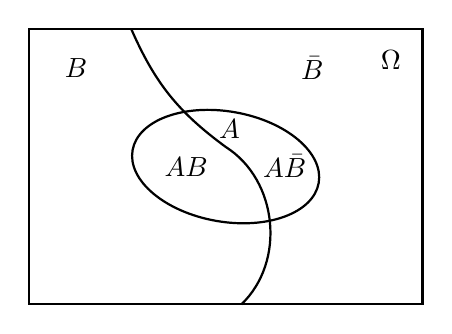
\begin{tikzpicture}[thick]
  \draw (0,0) rectangle (5,3.5);
  \node at (4.6,3.1) {$\Omega$};
  \node at (0.6,3) {$B$};
  \node at (3.6,3) {$\bar B$};
  \node at (2,1.75) {$AB$};
  \node at (3.25,1.75) {$A\bar B$};
  \node at (2.55,2.23) {$A$};
  \draw[rotate around={-10:(2.5,1.75)}]
    (2.5,1.75) ellipse (1.2 and 0.7);
  \draw (1.3,3.5) [bend right=15] to (2.5,2)
  [bend left=52] to (2.7,0);

\end{tikzpicture}
    \caption{用 $B$ 和 $\overline{B}$ 来分割样本空间}
  \end{minipage}
\end{figure}

\begin{example}[摸彩模型]
  设在 $n$ 张彩票中有一张奖券.
  求第二人摸到奖券的概率是多少?
\end{example}

\begin{solution}
  设 $A_i$ 表示事件“第 $i$ 人摸到奖券”,
  $i=1,2,\dotsc,n$,
  现在目的是求 $P(A_2)$.
  因为 $A_1$ 是否发生直接关系到 $A_2$ 发生的概率,
  即
  \[
    P(A_2 | A_1) = 0, \quad P(A_2 | A_1) = \frac{1}{n-1},
  \]
  而 $A_1$ 与 $\overline{A}_1$ 是两个概率大于 0 的事件:
  \[
    P(A_1) = \frac{1}{n}, \quad P(\overline{A}_1) = \frac{n-1}{n}.
  \]
  于是由全概率公式得
  \begin{align*}
    P(A_2)
    &= P(A_1) P(A_2 | A_1) + P(A_1) P(A_2 | \overline{A}_1)\\
    &= \frac{1}{n}.
  \end{align*}

  用类似的方法可得
  \[
    P(A_3) = P(A_4) = \dotsb = P(A_n) = \frac{1}{n}.
  \]

  如果设 $n$ 张彩票中有 $k(\le n)$ 张奖券,
  则可得
  \[
    P(A_1) = P(A_2) = \dotsb = P(A_n) = \frac{k}{n}.
  \]
  这说明,
  购买彩票时,
  不论先买后买,
  中彩机会是均等的.
\end{solution}

\begin{example}[敏感性问题调查]
  学生阅读黄色书刊和观看黄色影像会严重影响学生身心健康发展.
  但这些都是避着教师与家长进行的,
  属个人隐私行为.
  现在要设计一个调查方案,
  从调查数据中估计出学生中阅读黄色书刊和观看黄色影像的比率 $p$.
\end{example}

像这类敏感性问题的调查是社会调查的一类,
如一群人中参加赌博的比率、吸毒人的比率、经营者中偷税漏税户的比率、学生中考试作弊的比率等等.

敏感性问趣的调查方案,
关键要使被调查者愿意作出真实回答又能保守个人秘密.
一且调查方案设计有误,
被调查者就会拒绝配合,
所得调查数据将失去真实性.
经过多年研究和实践,
一些心理学家和统计学家设计了一种调查方案,
在这个方案中被调查者只需回答以下两个问题中的一个问题,
而且只需回答“是”或“否”.

\textbf{问题A}:
你的生日是否在7月1日之前?

\textbf{问题B}:
你是否看过黄色书刊或影像?

这个调查方来看似简单,
但为了消除被调查者的顾虑,
使被调查者确信他这次调查不会泄露个人秘密,
在操作上有以下关键点:
\begin{enumerate}
  \item 被调查者在没有旁人的情况下,
  独自一人回答问题.

  \item 被调查者从一个罐子中随机抽一只球,
  看过颜色后即放回.
  若抽到白球,
  则回答问题 A;
  若抽到红球,
  则回答问题 B.
  且罐中只有白球和红球.
\end{enumerate}

被调查者无论回答问题 A 或问题 B,
只需在下面答卷上认可的方框内打钩,
然后把答卷放入一只密封的投票箱内.

\begin{figure}
  \centering
  \begin{tikzpicture}[thick]
  \draw (0,0) rectangle (5,3.5);
  \node at (2.5,2.6) {答\,案};
  \node[draw ,rectangle] at (1.5,1.2) {};
  \node[draw ,rectangle] at (3.5,1.2) {};
  \node[left] at (1.5,1.2) {是};
  \node[left] at (3.5,1.2) {否};
\end{tikzpicture}
  \caption{敏感性问题的答卷}\label{fig1.4.4}
\end{figure}

如此的调查方法,
主要在于旁人无法知道被调查回答的是问题 A 还是问题 B,
由此可以极大地消除被调查者的顾虑.

现在的问题是如何分析调查的结果.
很显然,
我们对问题 A 是不感兴趣的.

首先我们设有 $n$ 张答卷 ($n$ 较大,
譬如 \num{1000} 以上),
其中有 $k$ 张回答“是”.
而我们又无法知道此 $n$ 张答卷中有多少张是回答问题 $B$ 的,
同样无法知道 $k$ 张回答“是”的答卷中有多少张是回答问题 $B$ 的.
但有两个信息我们是预先知道的,
即
\begin{enumerate}
  \item 在参加人数较多的场合,
  任选一人其生日在7月1日之前的概率为 0.5.

  \item 罐中红球的比率 $\pi$ 是已知.
  现在就要从这4个数据 $(n, k, 0.5, \pi)$ 去求出 $p$.
  因为由全概率公式得
  \[
    P(\text{是}) = P(\text{白球}) P(\text{是} | \text{白球})
    + P(\text{红球}) P(\text{是} | \text{红球}).
  \]
  所以将 $P(\text{红球}) = \pi$,
  $P(\text{白球}) = 1-\pi$,
  $P(\text{是} | \text{白球}) = 0.5$,
  $P(\text{是} | \text{红球}) = p$ 代入上式右边,
  而上式左边用频率 $k/n$ 代替,
  得
  \[
    \frac{k}{n} = 0.5 (1 - \pi) + p \cdot \pi.
  \]
  由此得
  \[
    p = \frac{k/n - 0.5(1 - \pi)}{\pi}
  \]
  因为我们用频率 $k/n$ 代替了概率 $P (\text{是})$,
  所以从上式得到的是 $p$ 的估计.
\end{enumerate}

例如,
在一次实际调查中,
罐中放有红球30个、白球20个,
则 $\pi = 0.6$,
调查结束后共收到 \num{1583} 张有效答卷,
其中有 389 张回答“是”,
由此可计算得
\[
  p = \frac{389/1583 - 0.5 \times 0.4}{0.6} = 0.0762.
\]
这表明:
约有 \SI{7.62}{\percent} 的学生看过黄色书刊或黄色影像.

\subsection{贝叶斯公式}

在乘法公式和全概率公式的基础上立即可推得一个很著名的公式.

\begin{property}[贝叶斯公式]\label{prop1.4.4}
  设 $B_1, B_2, \dotsc, B_n$ 是样本空间 $\Omega$ 的一个分割,
  即 $B_1, B_2, \dotsc, B_n$ 互不相容,
  且 $\bigcup_{i=1}^n B_i = \Omega$,
  如果 $P(A) > 0$, $P(B_i) > 0$, $i = 1,2, \dotsc, n$,
  则
  \begin{equation}
    P (B_i | A) = \frac{P(B_i) P(A|B_i)}{\sum_{j=1}^n P(B_j) P(A|B_j)},
    i = 1,2,\dotsc,n.
    \label{eq1.4.6}
  \end{equation}
\end{property}

\begin{proof}
  由条件概率的定义
  \[
    P(B_i|A) = \frac{P(AB_i)}{P(A)}.
  \]
  对上式的分子用乘法公式、分母用全概率公式,
  \begin{align*}
    & P(AB_i) = P(B_i) P(A|B_i),\\
    & P(A) = \sum_{j=1}^n P(B_j) P(A|B_j),
  \end{align*}
  即得
  \[
    P(B_i|A) = \frac{P(B_i) P(A|B_i)}{\sum_{j=1}^n P(B_j) P(A|B_j)}.
  \]
  结论得证.
\end{proof}

\begin{example}
  某地区居民的肝癌发病率为 \num{0.0004},
  现用甲胎蛋白法进行普查.
  医学研究表明,
  化验结果是存有错误的.
  已知患有肝癌的人其化验结果 \SI{99}{\percent} 呈阳性 (有病),
  而没患肝癌的人其化验结果 \SI{99.9}{\percent} 呈阴性 (无病).
  现某人的检查结果呈阳性,
  问他真的患肝癌的概率是多少?
\end{example}

\begin{solution}
  记 $B$ 为事件“被检查者患有肝癌”,
  $A$ 为事件“检查结果呈阳性”.
  由题设知
  \begin{gather*}
    P(B) = 0.0004, \quad P(\overline{B}) = 0.996,\\
    P(A|B) = 0.99, \quad P(A|\overline{B}) = 0.001.
  \end{gather*}

  我们现在的目的是求 $P(B|A)$.
  由贝叶斯公式得
  \begin{align*}
    P(B|A) &= \frac{P(B) P(A|B)}{P(B) P(A|B) + P(\overline{B}) P(A|\overline{B})}\\
    &= \frac{0.0004 \times 0.99}{0.0004 \times 0.99 + 0.9996 \times 0.001}\\
    &= 0.284.
  \end{align*}
  这表明,
  在检查结果呈阳性的人中,
  真患肝癌的人不到 \SI{30}{\percent},
  这个结果可能会使人吃惊,
  但仔细分析一下就可以理解了.
  因为肝癌发病率很低,
  在 \num{10000} 个人中,
  约有 4 人,
  而约有 \num{9996} 个人不惠肝癌.
  对 \num{10000} 个人用甲胎蛋白法进行检查,
  按其错检的概率可知,
  \num{9996} 个不患肝癌者中约有 $9996 \times 0.001 \cong 9.994$ 个呈阳性.
  另外 4 个真患肝癌者的检查报告中约有 $4 \times 0.99 \cong 3.96 $ 个呈阳性.
  仅从 \num{13.956} 个呈阳性者中看,
  真患肝癌的 3.96 人约占 \SI{28.4}{\percent}.
\end{solution}

进一步降低错检的概率是提高检验精度的关键.
在实际中由于技术和操作等种种原因,
降低错检的概率又是很困难的.
所以在实际中,
常采用复查的方法来减少错误率.
或用另一些简单易行的辅助方法先进行初查,
排除了大量明显不是肝癌的人后,
再用甲胎蛋白法对被怀疑的对象进行检查.
此时被怀疑的对象群体中,
肝癌的发病率已大大提高了.
警如,
对首次检查得阳性的人群再进行复查,
此时 $P(B) = 0.284$,
这时再用贝叶斯公式计算得
\[
  P(B|A) = \frac{0.284 \times 0.99}{0.284 \times 0.99 + 0.716 \times 0.0001} = 0.997.
\]
这就大大提高了甲胎蛋白法的准确率了.

在上面例中,
如果我们将事件 $B$ (“被检查者患有肝癌”) 看作是“原因”,
将事件 $A$ (“检查结果呈阳性”) 看作是最后“结果”.
则我们用贝叶斯公式在已知“结果”的条件下,
求出了“原因”的概率 $P(B|A)$.
而求“结果”的 (无条件) 概率 $P(A)$,
用全概率公式.
在上例中若取 $P(B) = 0.284$,
则
\begin{align*}
  P(A) &= P(B) P(A|B) + P(\overline{B}) P(A|\overline{B})\\
  &= 0.284 \times 0.99 + 0.716 \times 0.001\\
  &= 0.2819.
\end{align*}


条件概率的三公式中,
乘法公式是求事件交的概率.
全概率公式是求一个复杂事件的概率,
而贝叶斯公式是求一个条件概率.

在贝叶斯公式中,
如果称 $P(B_i)$ 为 $B_i$ 的先验概率,
称 $P(B_i |A)$ 为 $B_i$ 的后验概率, 则贝叶斯公式是专门用于计算后验概率的, 也就是通过$A$的发生这个新信息, 来对$B_i$的概率作出的修正. 下面例子很好地说明了这一点.

\begin{example}
  伊索寓言“孩子与狼”讲的是一个小孩每天到山上放羊,山里有狼出没.第一天,他在山上喊:“狼来了!狼来了!”,山下的村民闻声便去打狼,可到山上,发现狼没有来;第二天仍是如此;第三天,狼真的来了,可无论小孩怎么喊叫,也没有人来救他,因为前二次他说了谎,人们不再相信他了.
\end{example}

现在用贝叶斯公式来分析此寓言中村民对这个小孩的可信程度是如何下降的.

首先记事件$A$为“小孩说谎”,记事件$B$为“小孩可信”.不妨设村民过去对这个小孩的印象为
\begin{equation}\label{eq1.4.7}
  P(B) = 0.8,\quad P(\bar B) = 0.2.
\end{equation}

我们现在用贝叶斯公式来求$P(B|A)$,亦即这个小孩说了一次谎后,村民对他可信程度的改变.

在贝叶斯公式中我们要用到概率$P(A|B)$和$P(A|\bar B)$,这两个概率的含义是:前者为“可信”$(B)$的孩子“说谎”$(A)$的可能性,后者为“不可信”$(\bar B)$的孩子“说谎”$(A)$的可能性.在此不妨设
\[
  P(A|B) = 0.1,\quad P(A|\bar B) = 0.5.
\]

第一次村民上山打狼,发现狼没有来,即小孩说了谎$(A)$.村民根据这个信息,对这个小孩的可信程度改变为(用贝叶斯公式)
\begin{align*}
  P(B|A) & = \frac{P(B)P(A|B)}{P(B)P(A|B) + P(\bar B)P(A|\bar B) } \\
  & = \frac{0.8\times0.1}{0.8\times0.1 + 0.2\times0.5} = 0.444.
\end{align*}

这表明村民上了一次当后,对这个小孩的可信程度由原来的0.8调整为
0.444,也就是 \eqref{eq1.4.7} 调整为
\begin{equation}\label{eq1.4.8}
  P(B) = 0.444,\quad P(\bar B) = 0.556.
\end{equation}
在此基础上,我们再一次用贝叶斯公式来计算$P(B|A)$,亦即这个小孩第二次说谎后,村民对他的可信程度改变为
\[
  P(B|A) = \frac{0.444\times0.1}{0.444\times0.1 + 0.556\times0.5} = 0.138.
\]

这表明村民们经过两次上当,对这个小孩的可信程度已经从0.8下降到了
0.138,如此低的可信度,村民听到第三次呼叫时怎么再会上山打狼呢?

这个例子启发人们:若某人向银行贷款,连续两次未还,银行还会第三次贷款给他吗?
\begin{xiti}
  \item 某班级学生的考试成绩数学不及格的占15\%,语文不及格的占5\%,这两门都不及格的占3\%.
  \begin{enumerate}
    \item 已知一学生数学不及格,他语文也不及格的概率是多少?
    \item 已知一学生语文不及格,他数学也不及格的概率是多少?
  \end{enumerate}

  \item 设一批产品中一、二、三等品各占60\%,30\%,10\%.从中任意取出一件,结果不是三等品,求取到的是一等品的概率.

  \item 掷两颗骰子,以$A$记事件“两颗点数之和为10”,以$B$记事件“第一颗点数小于第二颗点数”,试求条件概率$P(A|B)$和$P(B|A)$.

  \item 设某种动物由出生活到10岁的概率为0.8,而活到15岁的概率为0.4.问现年为10岁的这种动物能活到15岁的概率是多少?

  \item 设10件产品中有4件不合格品,从中任取两件,已知其中一件是不合格品,求另一件也是不合格品的概率.

  \item 设$n$件产品中有$m$件不合格品,从中任取两件,已知两件中有一件是不合格品,求另一件也是不合格品的概率.

  \item 掷一颗骰子两次,以$x$,$y$分别表示先后掷出的点数,记
    \[
      A = \{ x + y = 10 \},\quad B = \{ x > y \},
    \]
    求$P(B|A),P(A|B)$.

  \item 已知$P(A)=1/4,P(B|A)=1/3,P(A|B)=1/2$,求$P(A\cup B)$.

  \item 已知$P(\bar A)=0.3,P(B)=0.4,P(A\bar B)=0.5$,求$P(B|A\cup \bar B)$.

  \item 设$A,B$为两事件,$P(A)=P(B)=1/3,P(A|B)=1/6$,求$P(\bar A|\bar B)$.

  \item 口袋中有1只白球,1只黑球.从中任取1只,若取出白球,则试验停止;若取出黑球,则把取出的黑球放回的同时,再加入1只黑球,如此下去,直到取出的是白球为止,试求下列事件的概率.
      \begin{enumerate}
        \item 取到第$n$次,试验没有结束;
        \item 取到第n次,试验恰好结束.
      \end{enumerate}

  \item 一盒晶体管中有6只合格品、4只不合格品.从中不返回地一只一只取出,试求第二次取出合格品的概率.

  \item 甲口袋有$a$只黑球、$b$只白球,乙口袋有$n$只黑球、$m$只白球.
      \begin{enumerate}
        \item 从甲口袋任取1只球放入乙口袋,然后再从乙口袋任取1只球.试求最后从乙口袋取出的是黑球的概率.
        \item 从甲口袋任取2只球放入乙口袋,然后再从乙口袋任取1只球.试求最后从乙口袋取出的是黑球的概率.
      \end{enumerate}

  \item 两台车床加工同样的零件,第一台出现不合格品的概率是0.03,第二台出现不合格品的概率是0.06,加工出来的零件放在一起,并且已知第一台加工的零件比第二台加工的零件多一倍.
      \begin{enumerate}
        \item 求任取一个零件是合格品的概率.
        \item 如果取出的零件是不合格品,求它是由第二台车床加工的概率.
      \end{enumerate}

  \item 已知男人中有5\%是色育患者,女人中有0.25\%是色盲患者,今从男女人数相等的人群中随机地挑选一人,发现恰好是色育患者,问此人是男性的概率是多少?

  \item 钥匙掉了,掉在宿舍里、掉在教室里、掉在路上的概率分别是40\%、30\%和20\%,而掉在上述三处地方被找到的概率分别是0.8、0.3和0.1.试求找到钥匙的概率.

  \item 口袋中有$a$个白球,$b$个黑球和$n$个红球,现从中一个一个不返回地取球.试证白球比黑球出现得早的概率为$a/(a+b)$,与$n$无关.

  \item 有两箱零件,第一箱装50件,其中10件是一等品;第二箱装30件,其中18件是一等品,现从两箱中随意挑出一箱,然而从该箱中任取两个零件,试求
      \begin{enumerate}
        \item 第一次取出的零件是一等品的概率;
        \item 在第一次取出的是一等品的条件下,第二次取出的零件仍然是一等品的概率.
      \end{enumerate}

  \item 学生在做一道有4个选项的单项选择题时,如果他不知道问题的正确答案时,就作随机猪测.现从卷面上看题是答对了,试在以下情况下求学生确实知道正确答案的概率.
      \begin{enumerate}
        \item 学生知道正确答案和胡乱猜测的概率都是$1/2$.
        \item 学生知道正确答案的概率是0.2.
      \end{enumerate}

  \item 口袋中有一只球,不知它的颜色是黑的还是白的.现再往口袋中放入一只白球,然后从口袋中任意取出一只,发现取出的是白球,试问口袋中原来那只球是白球的可能性为多少?

  \item 将$n$根绳子的$2n$个头任意两两相接,求恰好结成$n$个圈的概率.

  \item $m$个人相互传球,球从甲手中开始传出,每次传球时,传球者等可能地把球传给其余$m-1$个人中的任何一个.求第$n$次传球时仍由甲传出的概率.

  \item 甲、乙两人轮流掷一颗骰子,甲先掷.每当某人掷出1点时,则交给对方掷,否则此人继续掷.试求第$n$次由甲掷的概率.

  \item 甲口袋有1只黑球、2只白球,乙口袋有3只白球.每次从两口袋中各任取一球,交换后放人另一口袋.求交换$n$次后,黑球仍在甲口袋中的概率.

  \item 假设只考虑天气的两种情况:有雨或无雨.若已知今天的天气情况,明天天气保持不变的概率为$p$,变的概率为$1-p$.设第一天无雨,试求第$n$天也无雨的概率.

  \item 设罐中有$b$个黑球、$r$个红球,每次随机取出一个球,取出后将原球放回,再加人$c(>0)$个同色的球.试证:第$k$次取到黑球的概率为$b/(b+r),k=1,2,\cdots$.

  \item 设$P(A)>)$,试证
    \[
      P(B|A) \ge 1 - \frac{P(\bar B)}{P(A)}.
    \]

  \item 若事件$A$与$B$互不相容,且$P(\bar B)\ne0$,证明
    \[
      P(A|\bar B) = \frac{P(A)}{1-P(B)}.
    \]

  \item 设$A$,$B$为任意两个事件,且$A\subset B,P(B)>0$,则成立
    \[
      P(A) \le P(A|B).
    \]

  \item 若$P(A|B)>P(A|\bar B)$,试证$P(B|A)>P(B|\bar A)$.

  \item 设$P(A)=p,P(B)=1-\varepsilon$,证明
    \[
      \frac{p-\varepsilon}{1-\varepsilon} \le P(A|B) \le \frac p{1-\varepsilon}.
    \]
\end{xiti}


\section{独立性}

独立性是概率论中又一个重要概念,利用独立性可以简化概率的计算.下面先讨论两个事件之间的独立性,然后讨论多个事件之间的相互独立性,最后讨论试验之间的独立性.

\subsection{两个事件的独立性}
两个事件之间的独立性是指:一个事件的发生不影响另一个事件的发生.这在实际问题中是很多的,譬如在掷两颗骰子的试验中,记事件$A$为“第一颗骰子的点数为1”,记事件$B$为“第二颗骰子的点数为4”.则显然$A$与$B$的发生是相互不影响的.

另外,从概率的角度看,事件$A$的条件概率$P(A|B)$与无条件概率$P(A)$的差别在于:事件$B$的发生改变了事件$A$发生的概率,也即事件$B$对事件$A$有某种“影响”. 如果事件$B$的发生对事件A的发生毫无影响,即有$P(A|B)=P(A)$. 由此又可推出$P(B|A)=P(B)$,即事件$A$发生对$B$也无影响,可见独立性是相互的,它们都等价于

\begin{equation}\label{eq1.5.1}
  P(AB) = P(A)P(B).
\end{equation}
另外对$P(B)=0$,或$P(A)=0$,\eqref{eq1.5.1} 式仍然成立.为此,我们用 \eqref{eq1.5.1} 式作为两个事件相互独立的定义.

\begin{definition}{}{1.5.1}
  如果 \eqref{eq1.5.1} 式成立,则称事件$A$与$B$\textbf{相互独立}\index{D!独立性!相互独立},简称$A$与$B$独立,否则称$A$与$B$\textbf{不独立}\index{D!独立性!不独立}或\textbf{相依}.\index{D!独立性!相依}
\end{definition}

在许多实际问题中,两个事件相互独立大多是根据经验(相互有无影响)来判断的,如上述掷两颗骰子问题中A与B的独立性.但在有些问题中,有时也用  \eqref{eq1.5.1} 式来判断两个事件间的独立性.

\begin{example}[事件独立的例子]

  \begin{inparaenum}[(1)]
    \item 从一副52张的扑克牌中任取1张,以$A$记事件“取到黑桃”,以$B$记事件“取到爱司”,则因为$P(A)=1/4,P(B)=4/52=1/13$,而$AB$表示“取到黑桃爱司”,故$P(AB)=1/52$,所以$A$与$B$相互独立.

    \item\label{ex1.5.1.2} 考虑有三个小孩的家庭,并设所有8种情况
      \[
        bbb, bbg, bgb, gbb, bgg, gbg, ggb ,ggg
      \]
      是等可能的,其中$b$表示男孩,$g$表示女孩. 以$A$记事件“家中男女孩都有”,以$B$记事件“家中至多一个女孩”.则因为$P(A)=6/8,P(B)=4/8$,而$AB$表示“家中恰有一个女孩”,故$P(AB)=3/8$,所以$A$与$B$相互独立.

    \item 当考察的家庭有两个小孩时,样本空间只含4个样本点,它们是
      \[
        bb ,bg , gb ,gg
      \]

      若事件$A$、$B$仍如 (\ref{ex1.5.1.2}) 所设,则$P(A)=2/4,P(B)=3/4$,而$P(AB)=2/4$,由于$P(AB)\ne P(A)P(B)$,所以$A$与$B$不独立.
  \end{inparaenum}
\end{example}

\begin{property}\label{prop1.5.1}
  若事件$A$与$B$独立,则$A$与$\bar B$独立;$\bar A$与$B$独立;$\bar A$与$\bar B$独立.
\end{property}
\begin{proof}
  由概率的性质知
  \[
    P(A\bar B) = P(A) - P(AB).
  \]
  又由$A$与$B$的独立性知
  \[
    P(AB) = P(A)P(B),
  \]
  所以
  \[
    P(A\bar B) = P(A) - P(A)P(B) = P(A) [1 - P(B)] = P(A)P(\bar B).
  \]
  这表明$A$与$\bar B$独立. 类似可证$\bar A$与$\bar B$独立,$\bar A$ 与$B$独立.
\end{proof}

\subsection{多个事件的相互独立性}
首先研究三个事件的相互独立性,对此我们先给出以下的
\begin{definition}{}{1.5.2}
  设$A,B,C$是三个事件,如果有
  \begin{equation}\label{eq1.5.2}
    \left\{
      \begin{aligned}
        & P(AB) = P(A) P(B), \\
        & P(AC) = P(A) P(C), \\
        & P(BC) = P(B) P(C),
      \end{aligned}
    \right.
  \end{equation}
  则称$A,B,C$\textbf{两两独立}\index{D!独立性!两两独立}. 若还有
  \begin{equation}\label{eq1.5.3}
    P(ABC) = P(A) P(B) P(C),
  \end{equation}
  则称$A,B,C$\textbf{相互独立}.\index{D!独立性!相互独立}
\end{definition}

由此我们可以定义三个以上事件的相互独立性.
\begin{definition}{}{1.5.3}
  设有$n$个事件$A_1,A_2,\cdots,A_n$,对任意的$1\le i<j<k\cdots\le n$,如果以下等式均成立
  \begin{equation}\label{eq1.5.4}
    \left\{
      \begin{aligned}
        & P(A_iA_j) = P(A_i) P(A_j), \\
        & P(A_iA_jA_k) = P(A_i) P(A_j) P(A_k), \\
        & \vdots \\
        & P(A_1A_2\cdots A_n) = P(A_1)P(A_2) \cdots P(A_n),
      \end{aligned}
    \right.
  \end{equation}
  则称此$n$个事件$A_1,A_2,\cdots,A_n$\textbf{相互独立}.
\end{definition}

从上述定义可以看出,$n$个相互独立的事件中的任意一部分内仍是相互独立的,而且任意一部分与另一部分也是独立的.与性质 \ref{prop1.5.1} 类似,可以证明:将相互独立事件中的任一部分换为对立事件,所得的诸事件仍为相互独立的.

\begin{example}
  设$A$,$B$,$C$三事件相互独立,试证$A\cup B$与$C$相互独立.
\end{example}
\begin{proof}
  因为
  \begin{align*}
    P\big(\big(A\cup B)C) & = P(AC \cup BC) = P(AC) + P(BC) - P(ABC) \\
    & = P(A)P(C) + P(B)P(C) - P(A)P(B)P(C) \\
    & = [P(A) + P(B) - P(A)P(B)]P(C) =
    P(A \cup B) P(C),
  \end{align*}
  所以$A\cup B$与$C$相互独立.
\end{proof}

仿照此题的证明,可很容易推得:$AB$与$C$独立;$A-B$与$C$独立.

\begin{example}
  两射手彼此独立地向同一目标射击,设甲射中目标的概率为0.9,乙射中目标的概率为0.8,求目标被击中的概率是多少?
\end{example}
\begin{solution}
  记$A$为事件“甲射中目标”,$B$为事件“乙射中目标”. 注意到事件“目标被击中”$=A\cup B$,故
  \begin{align*}
    P(A\cup B) & = P(A) + P(B) - P(A)P(B) \\
    & = 0.9 + 0.8 - 0.9\times 0.8 = 0.98.
  \end{align*}
\end{solution}

\begin{example}
  某零件用两种工艺加工,第一种工艺有三道工序,各道工序出现不合格品的概率分别为$0.3,0.2,0.1$;第二章工艺有两道工序,各道工序出现不合格品的概率分别为$0.3,0.2$. 试问:
  \begin{enumerate}[label=(\arabic*)]
    \item 用哪种工艺加工得到合格品的概率较大些?
    \item 第二种工艺两道工序出现不合格品的概率都是0.3时,情况又如何?
  \end{enumerate}
\end{example}

\begin{solution}
  以$A_i$记事件“用第$i$种工艺加工得到合格品”,$i=1,2$.

  \begin{inparaenum}[(1)]
    \item 由于各道工序可看作是独立工作的,所以
    \begin{align*}
      & P(A_1) = 0.7\times 0.8 \times 0.9 = 0.504, \\
      & P(A_2) = 0.7\times 0.8 = 0.56,
    \end{align*}
    即第二种工艺得到合格品的概率较大些. 这个结果也是可以理解的,因为第二种工艺前两道工序出现不合格品的概率与第一种工艺相同,但少了一道工序,所以减少了出现不合格品的机会.

    \item 当第二种工艺两道工序出现不合格品的概率都是0.3时,
    \[
      P(A_2) = 0.7\times 0.7 = 0.49,
    \]
    即第一种工艺得到合格品的概率较大些.
  \end{inparaenum}
\end{solution}

\begin{example}
  有两名选手比赛射击,轮流对同一目标进行射击,甲命中目标的概率为$\alpha$,乙命中目标的概率为$\beta$.甲先射,谁先命中谁得胜.问甲、乙两人获胜的概率各为多少?
\end{example}
\begin{solution}
  记事件$A_i$为“第i次射击命中目标”,$i=1,2$,因为甲先射,所以事件“甲获胜”可以表示为
  \[
    A_1 \cup \bar A_1\bar A_2 A_3 \cup \bar A_1\bar A_2
    \bar A_3\bar A_4A_5\cup\cdots,
  \]
  又因为各次射击是独立的,所以得
  \begin{align*}
    P(\,\text{甲获胜}\,) & = \alpha + (1-\alpha)(1-\beta)\alpha + (1-\alpha)^2(1-\beta)^2\alpha + \cdots \\
    & = \alpha\sum_{i=0}^{+\infty}(1-\alpha)^i(1-\beta)^i \\
    & = \frac{\alpha}{1-(1-\alpha)(1-\beta)}.
  \end{align*}
  同理可得
  \begin{align*}
    P(\,\text{乙获胜}\,) & = P (\bar A_1A_2\cup \bar A_1\bar A_2\bar A_3A_4\cup\cdot) \\
    & = (1-\alpha)\beta + (1-\alpha)(1-\beta)(1-\alpha)\beta + \cdots \\
    & \beta (1-\alpha)\sum_{i=0}^{+\infty}(1-\alpha)^i(1-\beta)^i \\
    & = \frac{\beta(1-\alpha)}{1-(1-\alpha)(1-\beta)}.
  \end{align*}
\end{solution}

此题在等比级数求和时,应该有条件:公比$|(1-\alpha)(1-\beta)|M1$. 这一点不难从题目的实际意义中得到. 因为对本题而言,$\alpha,\beta$取值为零或1均是无意义的.

\begin{example}
  系统由多个元件组成,且所有元件都独立地工作.设每个元件正常工作的概率都为$p=0.9$,试求以下系统正常工作的概率.
  \begin{enumerate}[label=(\arabic*)]
    \item 串联系统$S_1$: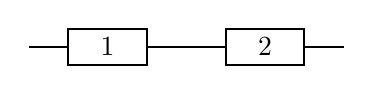
\begin{tikzpicture}[baseline=(a.base),thick]
                       \draw (0,0) -- (4,0);
                       \node(a)[minimum width=1cm,minimum height=0.4cm,draw,fill=white] at (1,0){1};
                       \node[minimum width=1cm,minimum height=0.4cm,draw,fill=white] at (3,0){2};
                    \end{tikzpicture}.
    \item 并联系统$S_2$: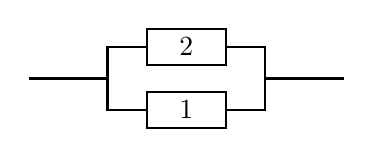
\begin{tikzpicture}[baseline=(a.base),thick,
     every node/.style =
     { minimum width=1cm,minimum height=0.4cm,draw,fill=white}]
     \node[draw = white](a) at (2,0) {};
     \draw (0,0) -- (1,0)  (3,0) -- (4,0)
         (1.5,-0.4) -- (1,-0.4) -- (1,0.4) -- (1.5,0.4)
          (2.5,-0.4) -- (3,-0.4) -- (3,0.4) -- (2.5,0.4);
     \node at (2,-0.4) {1} ;
     \node at (2,0.4) {2} ;
   \end{tikzpicture}.
   \item 5个元件组成的桥式系统$S_3$: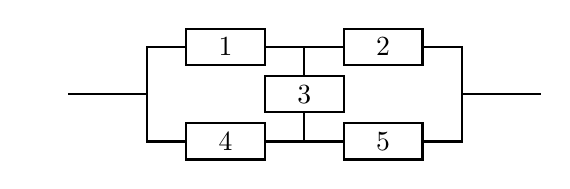
\begin{tikzpicture}[baseline=(a.base),thick,
  every node/.style =
   { minimum width=1cm,minimum height=0.4cm,draw,fill=white}]
   \node[draw = white] (a) at (0,0) {};
   \draw (0,0) -- (1,0) (3,-0.6) -- (3,0.6) (5,0) -- (6,0)
         (1,0.6) -- (1,-0.6) -- (5,-0.6) -- (5,0.6) -- cycle;
   \node at (2,-0.6) {4};
   \node at (2,0.6) {1};
   \node at (3,0) {3};
   \node at (4,0.6) {2};
   \node at (4,-0.6) {5};
\end{tikzpicture}.
  \end{enumerate}
\end{example}

\begin{solution}
  设$S_i=$“第$i$个系统正常工作”,$A_i=$“第$i$个元件正常工作”.

  \begin{inparaenum}[(1)]
    \item 对申联系统而言,“系统正常工作”相当于“所有元件正常工作”,即$S_1=A_1A_2$,所以
        \[
          P(S_1) = P(A_1A_2) = P(A_1)P(A_2) = p^2 = 0.81.
        \]

        这也可看出:两个正常工作概率为0.9的元件组成的串联系统,其系统正常工作的概率下降为0.81.

    \item 对并联系统而言,“系统正常工作”相当于“至少一个元件正常工作”,即$S_2=A_1\cup A_2$,所以
        \begin{align*}
          P(S_2) & P(A_1\cup A_2) = P(A_1) + P(A_2) - P(A_1A_2) \\
          & = p + p - p^2 = 0.99.
        \end{align*}
        或
        \begin{align*}
          P(S_2) & = 1 - P(\bar S_2) = 1 - P(\bar{A_1\cup A_2}) = 1 - P(\bar A_1\cap \bar A_2) \\
          & = 1 - P(\bar A_1)P(\bar A_2) = 1 - (1-p)^2 = 0.99.
        \end{align*}
        这也可看出:两个正常工作概率为0.9的元件组成的并联系统,其系统正常工作的概率提高至0.99.

        \item 在桥式系统中,第3个元件是关键,我们先用全概率公式得
        \[
          P(S_3) = P(A_3)P(S_3|A_3) + P(\bar A_3)P(S_3|\bar A_3).
        \]
        因为在“第3个元件正常工作”的条件下,系统成为先并后串系统(见图 \ref{fig1.5.1}). 所以
        \begin{align*}
          P(S_3|A_3) & = P\big( ( A_1\cup A_4 )
          (A_2 \cup A_5) \big) = P(A_1\cup A_4)P(A_2\cup A_5) \\
          & = [ 1 - (1-p)^2 ]^2 = 0.9801.
        \end{align*}

        又因为在“第3个元件不正常工作”的条件下,系统成为先串后并系统(见图 \ref{fig1.5.2}).
  \end{inparaenum}
  \begin{figure}[!ht]
    \centering
    \begin{minipage}{0.48\linewidth}
      \centering
      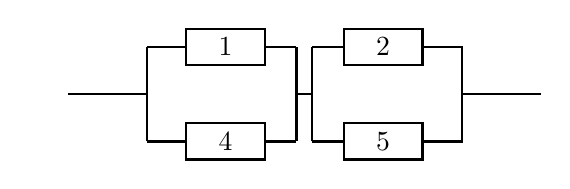
\begin{tikzpicture}[baseline=(a.base),thick,
  every node/.style =
   { minimum width=1cm,minimum height=0.4cm,draw,fill=white}]
   \node[draw = white] (a) at (0,0) {};
   \draw (0,0) -- (1,0) (2.9,0) -- (3.1,0)
    (5,0) -- (6,0) (2.9,-0.6) -- (2.9,0.6)
    (3.1,-0.6) -- (3.1,0.6)
         (1,0.6) -- (1,-0.6)(2.9,-0.6) (3.1,-0.6)-- (5,-0.6) -- (5,0.6) -- (3.1,0.6) (2.9,0.6) -- cycle;
    \draw (1,0.6) -- (2.9,0.6) (1,-0.6) -- (2.9,-0.6);
   \node at (2,-0.6) {4};
   \node at (2,0.6) {1};
   \node at (4,0.6) {2};
   \node at (4,-0.6) {5};
   \end{tikzpicture}
   \caption{先并后串系统\label{fig1.5.1}}
    \end{minipage}%
    \begin{minipage}{0.48\linewidth}
      \centering
      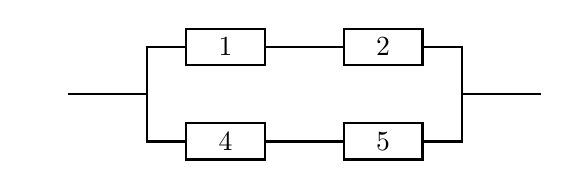
\begin{tikzpicture}[baseline=(a.base),thick,
  every node/.style =
   { minimum width=1cm,minimum height=0.4cm,draw,fill=white}]
   \node[draw = white] (a) at (0,0) {};
   \draw (0,0) -- (1,0)  (5,0) -- (6,0)
         (1,0.6) -- (1,-0.6) -- (5,-0.6) -- (5,0.6) -- cycle;
   \node at (2,-0.6) {4};
   \node at (2,0.6) {1};
   \node at (4,0.6) {2};
   \node at (4,-0.6) {5};
\end{tikzpicture}
   \caption{先串后并系统\label{fig1.5.2}}
    \end{minipage}
  \end{figure}
  所以
  \[
    P(S_3|\bar A_3) = P(A_1A_2|\cup A_4A_5) = 1 - (1-p^2)^2 = 0.9639.
  \]
  最后我们得
  \begin{align*}
    P(S_3) & = p [ 1-(1-p)^2 ]^2 + (1-p)[ 1-(1-p^2)^2 ] \\
    & = 0.9\times 0.9801 + 0.1 \times 0.9639 = 0.9785.
  \end{align*}
\end{solution}

\subsection{试验的独立性}
利用事件的独立性可以定义两个或更多个试验的独立性.

\begin{definition}{}{1.5.4}
  设有两个试验$E_1$和$E_2$,假如试验$E_1$的任一结果(事件)与试验$E_2$的任一结果(事件)都是相互独立的事件,则称\textbf{这两个试验相互独立}.
\end{definition}

例如掷一枚硬币(试验$E_1$)与掷一颗骰子(试验$E_2$)是相互独立的试验.

类似地可以定义$n$个试验$E_1,E_2,\cdots,E_n$的相互独立性:如果$E_1$的任一结果、$E_2$的任一结果$\cdots\cdots E_n$的任一结果都是相互独立的事件,则称\textbf{试验$E_1,E_2,\cdots,E_n$相互独立}. 如果这$n$个独立试验还是相同的,则称其为\textbf{$n$重独立重复试验}. 如果在$n$重独立重复试验中,每次试验的可能结果为两个:$A$或$\bar A$,则称这种试验为\textbf{$n$重伯努利试验}. \index{B!伯努利试验}

例如掷$n$枚硬币、掷$n$颗骰子、检查$n$个产品等,都是$n$重独立重复试验.

\begin{example}
  某彩票每周开奖一次,每次提供十万分之一的中奖机会,且各周开奖是相互独立的.若你每周买一张彩票,尽管你坚持十年(每年52周)之久,你从未中奖的可能性是多少?
\end{example}

\begin{solution}
  按假设,每次中奖的可能性是$10^{-5}$,于是每次不中奖的可能性是$1-10^{-5}$. 另外,十年中你共购买彩票520次,每次开奖都是相互独立的,相当于进行了520次独立重复试验.记$A_i$为“第$i$次开奖不中奖”,$i=1,2,\cdots,520$,则$A_1,A_2,\cdots,A_{520}$相互独立,由此得十年中你从未中奖的可能性是
  \[
    P(A_1A_2\cdots A_{520}) = (1 - 10^{-5})^{520} =  0.9948.
  \]
  这个概率表明十年中你从未中奖是很正常的事.
\end{solution}

如果将上例中每次中奖机会改成“万分之一”,则十年中从未中奖的可能性还是很大的,为0.9493.

\begin{xiti}
  \item 三人独立地破译一个密码,他们能单独译出的概率分别为$1/5$,$1/3$,$1/4$,求此密码被译出的概率.

  \item 有甲乙两批种子,发芽率分别为0.8和0.7,在两批种子中各任取一粒,求:
      \begin{enumerate}
        \item 两粒种子都能发芽的概率;
        \item 至少有一粒种子能发芽的概率;
        \item 恰好有一粒种子能发芽的概率.
      \end{enumerate}

  \item 甲、乙两人独立地对同一目标射击一次,其命中率分别为0.6和0.7,现已知目标被击中,求它是甲射中的概率.

  \item 设电路由$A$,$B$,$C$三个元件组成,若元件$A$,$B$,$C$发生故障的概率分别是0.3,0.2,0.2,且各元件独立工作,试在以下情况下,求此电路发生故障的概率:
      \begin{enumerate}
        \item $A$,$B$,$C$三个元件串联;
        \item $A$,$B$,$C$三个元件并联;
        \item 元件$A$与两个并联的元件$B$及$C$串联而成.
      \end{enumerate}

  \item 在一小时内甲,乙,丙三台机床需维修的概率分别是0.9,0.8和0.85,求一小时内
      \begin{enumerate}
        \item 没有一台机床需要维修的概率;
        \item 至少有一台机床不需要维修的概率;
        \item 至多只有一台机床需要维修的概率.
      \end{enumerate}

  \item 设$A_1,A_2,A_3$相互独立,且$P(A_i)=1/3,i=1,2,3$. 试求$A_1,A_2,A_3$中
      \begin{enumerate}
        \item 至少出现一个的概率;
        \item 恰好出现一个的概率;
        \item 最多出现一个的概率.
      \end{enumerate}

  \item 若事件$A$与$B$相互独立且互不相容,试求$\min\{P(A),P(B)\}$.

  \item 假设$P(A)=0.4,P(A\cup B)=0.7$,在以下情况下求$P(B)$:
      \begin{enumerate}
        \item $A,B$互不相容;
        \item $A,B$独立;
        \item $A\subset B$.
      \end{enumerate}

  \item 设$A,B,C$两两独立,且$ABC=\varnothing$.
      \begin{enumerate}
        \item 如果$P(A)=P(B)=P(C)=x$,试求$x$的最大值;
        \item 如果$P(A)=P(B)=P(C)<1/2$,且$P(A\cup B\cup C)=9/16$,求$P(A)$.
      \end{enumerate}

  \item 事件$A,B$独立,两个事件仅$A$发生的概率或仅$B$发生的概率都是$1/4$,求$P(A)$及$P(B)$.

  \item 一实习生用同一台机器接连独立地制造3个同种零件,第$i$个零件是不合格品的概率为$p_i=1/(i+1),i=1,2,3$,以$X$表示3个零件中合格品的个数,求$P(X=2)$.

  \item 同时抛掷3枚均匀的硬币,试求恰好有两枚正面向上的概率.

  \item 一射手对同一目标独立地进行四次射击,若至少命中一次的概率为80/81,试求该射手进行-一次射击的命中率.

  \item 每次射击命中率为0.2,试求:射击多少次才能使至少击中一次的概率不小于0.9?

  \item 设猎人在猎物100米处对猎物打第一枪,命中猎物的概率为0.5.若第一枪未命中,则猎人继续打第二枪,此时猎物与猎人已相距150米.若第二枪仍未命中,则猎人继续打第三枪,此时猎物与猎人已相距200米.若第三枪还未命中,则猎物逃逸.假如该猎人命中猎物的概率与距离成反比,试求该猎物被击中的概率.

  \item 已知某商场一天内来$k$个顾客的概率为$\lambda^k\ee^{-\lambda}/k!,k=0,1,\cdots$,其中$\lambda>0$. 又设每个到达商场的顾客购买商品是独立的,其概率为$p$,试证:这个商场一天内有$r$个顾客购买商品的概率为:$(\lambda p)^r\ee^{-\lambda p}/r!$.

  \item 一个人的血型为$A$,$A$,$AB$,$O$型的概率分别为0.37,0.21,0.08,0.34.现任意挑选四个人,试求:
      \begin{enumerate}
        \item 此四人的血型全不相同的概率;
        \item 此四人的血型全部相同的概率.
      \end{enumerate}

  \item 甲、乙两选手进行乓球单打比赛,已知在每局中甲胜的概率为0.6,乙胜的概率为0.4. 比赛可采用三局二胜制或五局三胜制,问哪一种比赛制度对甲更有利?

  \item 甲、乙、丙三人进行比赛,规定每局两个人比赛,胜者与第三人比赛,依次循环,直至有一人连胜两次为止,此人即为冠军.而每次比赛双方取胜的概率都是1/2,现假定甲、乙两人先比,试求各人得冠军的概率.

  \item 甲、乙两个赌徒在每一局获胜的概率都是1/2.两人约定谁先赢得一定的局数就获得全部赌本.但赌博在中途被打断了,请问在以下各种情况下,应如何合理分配赌本:
      \begin{enumerate}
        \item 甲、乙两个赌徒都各需赢$k$局才能获胜;
        \item 甲赌徒还需赢2局才能获胜,乙赌徒还需赢3局才能获胜;
        \item 甲赌徒还需赢$n$局才能获胜,乙赌徒还需赢$m$局才能获胜.
      \end{enumerate}

  \item 试证:概率为零的事件与任何事件都是独立的.

  \item 设$A,B,C$三事件相互独立,试证$A-B$与$C$独立.

  \item 设$0<P(B)<1$,试证事件$A$与$B$独立的充要条件是
  \[
    P(A|B) = P(A|\bar B).
  \]

  \item 设$0<P(A)<1,0<P(B)<1,P(A|B)+P(\bar A|\bar B)=1$,试证$A$与$B$独立.

  \item 若$P(A)>0,P(B)>)$,如果$A,B$相互独立,试证$A,B$相容.
\end{xiti} 